% Paquets généraux
\documentclass[a4paper,12pt,titlepage,twoside]{article}
\usepackage[T1]{fontenc}
\usepackage[utf8]{inputenc}
\usepackage[french]{babel}
\usepackage{subcaption}
\addto\captionsfrench{%
  \renewcommand{\tablename}{Tableau}%
}
\usepackage[gen]{eurosym}
%\usepackage[dvips]{graphicx}
\usepackage{minted}
\usepackage{fancyhdr}
\usepackage{pdfpages} 
\usepackage{multido}
\usepackage{hyperref}
\usepackage{textcomp}
\usepackage{schemabloc}
%\usepackage[bitstream-charter]{mathdesign}
\usepackage{array}
\newcolumntype{P}[1]{>{\centering\arraybackslash}p{#1}}
\usepackage[shortlabels]{enumitem}
\usepackage[framemethod=TikZ]{mdframed}

\newcommand{\id}{71}
\newcommand{\nom}{Théorie des mécanismes}
\newcommand{\sequence}{04}
\newcommand{\nomsequence}{Liaisons entre les solides}
\newcommand{\num}{02}
\newcommand{\type}{KH}
\newcommand{\descrip}{Liaisons équivalentes, hyperstatisme, liaisons en série et en parallèle, théorie des graphes}
\newcommand{\competences}{B2-12: Proposer une modélisation des liaisons avec leurs caractéristiques géométriques. \\ &  B2-13: Proposer un modèle cinématique paramétré à partir d'un système réel, d'une maquette numérique ou d'u \\ &  B2-17: Simplifier un modèle de mécanisme. \\ &  B2-18: Modifier un modèle pour le rendre isostatique. \\ &  C1-04: Proposer une démarche permettant d'obtenir une loi entrée-sortie géométrique.  \\ &  C2-05: Caractériser le mouvement d'un repère par rapport à un autre repère. \\ &  C2-06: Déterminer les relations entre les grandeurs géométriques ou cinématiques. }
\newcommand{\nbcomp}{7}
\newcommand{\systemes}{}
\newcommand{\systemesnum}{}
\newcommand{\systemessansaccent}{}
\newcommand{\ilot}{2}
\newcommand{\ilotstr}{02}
\newcommand{\dossierilot}{\detokenize{Ilot_02 }}

%\usepackage{style}
\usepackage{bodegraph}
\usepackage{rpcinematik}
\usepackage[locale = FR]{siunitx}
\usepackage{caption}
\newcommand{\institute}{Lycée Dorian}

\usepackage{listings}
\usepackage{fancyvrb}
\usepackage{color}
\usepackage{xcolor}
\usepackage{colortbl}
\usepackage{helvet}
\usepackage[frenchmath]{newtxsf} % for sans serif symbols
\renewcommand{\familydefault}{\sfdefault}
%\usepackage{amsfonts}
%\usepackage{amsmath}
%\usepackage{lmodern}
\usepackage{mathastext}
%\usepackage{xspace}
\usepackage{varioref}
\usepackage{tabularx}
%\usepackage{floatflt}
\usepackage{graphics}
\usepackage{wrapfig}
\usepackage{textcomp}
\usepackage{tikz,tkz-tab}
\usepackage[european resistor, european voltage, european current]{circuitikz}
\usepackage{wrapfig}
\usepackage{gensymb}
\usepackage[percent]{overpic}
\usetikzlibrary{babel}
\usepackage{ifthen}
\usepackage{cancel}
\usepackage{etoolbox}
\usepackage{multirow}
%\usepackage{boxedminipage}
\definecolor{gris25}{gray}{0.75}
\definecolor{bleu}{RGB}{18,33,98}
\definecolor{bleuf}{RGB}{42,94,171}
\definecolor{bleuc}{RGB}{231,239,247}
\definecolor{bleum}{RGB}{160,195,226}
\definecolor{rougef}{RGB}{185,18,27}
\definecolor{rougec}{RGB}{255,188,204}%255,230,231
\definecolor{vertf}{RGB}{103,126,82}
\definecolor{vertc}{RGB}{220,255,191}
\definecolor{forestgreen}{rgb}{0.13,0.54,0.13}
\definecolor{blcr}{rgb}{0.59,0.69,0.84}
\definecolor{blfr}{rgb}{0.32,0.51,0.75}
\definecolor{orfr}{rgb}{0.90,0.42,0.15}
\definecolor{orcr}{rgb}{0.90,0.65,0.50}
\definecolor{orangef}{rgb}{0.659,0.269,0.072}
\definecolor{orange}{rgb}{0.58,0.35,0.063}
\definecolor{orangec}{rgb}{0.43,0.32,0.25}
\definecolor{rcorrect}{rgb}{0.6,0,0}
\definecolor{sequence}{rgb}{0.75,0.75,0.75}
\definecolor{competences}{rgb}{0.61,0.73,0.35}
\definecolor{rose}{HTML}{ff00ff}
\definecolor{grisf}{HTML}{222222}
\definecolor{grisc}{HTML}{636363}
\definecolor{normal}{HTML}{4087c4}
\definecolor{info}{HTML}{5bc0de}
\definecolor{success}{RGB}{92,184,92}
\definecolor{warning}{RGB}{240,173,78}
\definecolor{danger}{RGB}{217,83,79}
\hypersetup{                    % parametrage des hyperliens
    colorlinks=true,                % colorise les liens
    breaklinks=true,                % permet les retours à la ligne pour les liens trop longs
    urlcolor= blfr,                 % couleur des hyperliens
    linkcolor= orange,                % couleur des liens internes aux documents (index, figures, tableaux, equations,...)
    citecolor= forestgreen                % couleur des liens vers les references bibliographiques
    }

\newcolumntype{M}[1]{>{\centering\arraybackslash}m{#1}}
\definecolor{codegreen}{rgb}{0,0.6,0}
\definecolor{codegray}{rgb}{0.5,0.5,0.5}
\definecolor{codepurple}{rgb}{0.58,0,0.82}
\definecolor{backcolour}{rgb}{0.95,0.95,0.92}

\lstdefinestyle{mystyle}{
    backgroundcolor=\color{backcolour},   
    commentstyle=\color{codegreen},
    keywordstyle=\color{magenta},
    numberstyle=\tiny\color{codegray},
    stringstyle=\color{codepurple},
    basicstyle=\ttfamily\footnotesize,
    breakatwhitespace=false,         
    breaklines=true,                 
    captionpos=b,                    
    keepspaces=true,                 
    numbers=left,                    
    numbersep=5pt,                  
    showspaces=false,                
    showstringspaces=false,
    showtabs=false,                  
    tabsize=2
}

\lstset{style=mystyle}

% Mise en page
\pagestyle{fancy}

\setlength{\hoffset}{-18pt}
\setlength{\oddsidemargin}{0pt} 	% Marge gauche sur pages impaire2s
\setlength{\evensidemargin}{0pt} 	% Marge gauche sur pages paires
\setlength{\marginparwidth}{00pt} 	% Largeur de note dans la marge
\setlength{\headwidth}{481pt} 	 	% Largeur de la zone de tête (17cm)
\setlength{\textwidth}{481pt} 	 	% Largeu\textbf{r de la zone de texte (17cm)
\setlength{\voffset}{-18pt} 		% Bon pour DOS
\setlength{\marginparsep}{7pt}	 	% Séparation de la marge
\setlength{\topmargin}{-30pt} 		% Pas de marge en haut
\setlength{\headheight}{55pt} 		% Haut de page
\setlength{\headsep}{20pt} 		% Entre le haut de page et le texte
\setlength{\footskip}{30pt} 		% Bas de\textbf{ page + séparation
\setlength{\textheight}{700pt} 		% Hauteur de l'icone zone de texte (25cm)
\setlength\fboxrule{1 pt}
\renewcommand{\baselinestretch}{1}
\setcounter{tocdepth}{1}
\newcommand{\cadre}[2]
{\fbox{
  \begin{minipage}{#1\linewidth}
   \begin{center}
    #2\\
   \end{center}
  \end{minipage}
 }
}

\newcommand{\repon}[1]
{
~\ \\
\begin{tabular}{|m{\linewidth}|}
 \hline
\multido{}{#1}{\\ \hline}
\end{tabular}
}


\newcommand{\objectif}[1]{
\mdfsetup{%
frametitle={%
\tikz[baseline=(current bounding box.east),outer sep=0pt]
\node[anchor=east,rectangle,fill=bleum]
{\strut Objectif~};}}
\mdfsetup{innertopmargin=10pt,linecolor=bleum,%
linewidth=2pt,topline=true,%
frametitleaboveskip=\dimexpr-\ht\strutbox\relax
}
\begin{mdframed}[]\relax%
#1
\end{mdframed}}


\newcounter{num_quest} \setcounter{num_quest}{0}
\newcounter{num_rep} \setcounter{num_rep}{0}
\newcounter{num_cor} \setcounter{num_cor}{0}

\newcommand{\feuilleDR}[1]{
	\begin{tikzpicture}
		\draw[gray!30](0,0)grid[step=0.5cm](\linewidth,#1);
	\end{tikzpicture}
}

%\newcommand{\question}[1]{\refstepcounter{num_quest}\par
%~\ \\ \parbox[t][][t]{0.15\linewidth}{\textbf{Question \arabic{num_quest}}}\parbox[t][][t]{0.85\linewidth}{#1\label{q\the\value{num_quest}}}\par
%}

\newcommand{\question}[1]{\refstepcounter{num_quest}\par
~\ \\ \textbf{Question \arabic{num_quest} : }#1\label{q\the\value{num_quest}}\par
}

\newcommand{\posetafigure}[3]{
\begin{figure}[ht!]
 \begin{center}
  \includegraphics[width=#2\linewidth]{img/#1}
 \end{center}
 \caption{\label{#1} #3}
\end{figure}}

\newcommand{\goforum}{
\begin{figure}

\end{figure}
\begin{center}
 
\includegraphics[width=0.7\linewidth]{../../../img/go_forum}
\end{center}
\label{go_forum}
\caption{J'pète les plombs}
\end{figure}}

\newcommand{\reponse}[4][1]
{\noindent
\parbox{\textwidth}{
\rule{\linewidth}{.5pt}\\
\textbf{Question\ifthenelse{#1>1}{s}{} \multido{}{#1}{%
\refstepcounter{num_rep}\ref{q\the\value{num_rep}} }:} ~\ \\
\ifdef{\public}{#3 \ifthenelse{#2>0}{~\ \\ 	\feuilleDR{#2}}}{#4}
}}

\newcommand{\cor}
{\refstepcounter{num_cor}
\noindent
\rule{\linewidth}{.5pt}
\textbf{Question \arabic{num_cor}:} \\
}

\newcommand{\finsujet}
{
    \begin{center}
    \Large{FIN}
    \end{center}

    \cleardoublepage

    \ifdef{\public}{\pagestyle{docreponse}}{\pagestyle{correction}}

    \ifdef{\public}{
        \begin{tikzpicture} 
            \draw (0,0) rectangle (2,2);
            \draw (0,0) -- (2,2);
            \draw (1.5,0.5) node {\large 20};
            \draw (2.5,0) rectangle (16,2);
            \draw (4.5,1.7) node {\large Commentaires:};
        \end{tikzpicture}
    }
    ~\ \\
}


%\newcommand{\repcarre}[2]
%{
%~\ \\
%\begin{tikzpicture}
%\draw [fill=white] (0,0) rectangle +(\linewidth,#1);
%\node[align=left] at (1.1,#2-0.3) {\textbf{Question #1:}};
%\end{tikzpicture}
%}

\newcommand{\titre}[1]
{\begin{center}
\cadre{0.8}{\huge #1} 
\end{center}
}


%Définition des torseurs :
\newcommand{\torseur}[2]{\left\{\mathcal{#1}_{#2} \right\}}
\newcommand{\torseurh}[3]{\left\{\genfrac{}{}{0pt}{0}{#1}{#2}\right\}_{#3}}
\newcommand{\torseurv}[8]{\left\{
\begin{matrix}
#1 & #4 \\ #2 & #5 \\ #3 &#6
\end{matrix}
\right\}_{{#7},{#8}}}

%Définition des torseurs :
%\newcommand{\torseur}[2]{\left \{\mbox{\relsize{2}{$\mathcal {#1}$}\relsize{-2}}\phantom{}_{\mbox{\scriptsize $#2$}} \right \}}
%\newcommand{\torseurh}[3]{\left\{\genfrac{}{}{0pt}{0}{#1}{#2}\right\}_{#3}}
%\newcommand{\torseurv}[8]{
%\left\{\begin{array}{@{}c|c@{}} #1 & #4 \\ #2 & #5 \\ #3 & #6 \end{array} \right\}_{#7,#8}
%}
\newcommand{\derivee}[2]{\left.\dfrac{\d #1}{\d t}\right|_{#2}}
\newcommand{\tripleint}{\int\!\!\!\!\!\int\!\!\!\!\!\int}

% Notation cinématique et statique
\newcommand{\cinematique}[2]{\mbox{#1}/\mbox{#2}}
\newcommand{\statique}[2]{\mbox{#1}\rightarrow\mbox{#2}}
\newcommand{\moment}[3]{\vv {#1}_{\scriptsize{#3}}(#2)}
\newcommand{\resultante}[2]{\vv {#1}_{\scriptsize{#2}}}


%Commande de base
\newcommand{\jo}{\left(j\omega\right)} % j \omega dans l'analyse fréquentielle
\newcommand{\tl}{\xrightarrow{\mathcal{L}}} % transformée de laplace sur fleche
\newcommand{\tli}{\xrightarrow{\mathcal{L}^{-1}}} % transformée inverse de laplace sur fleche
\renewcommand{\d}[1][]{\mathrm{d#1}}
\newcommand{\dd}[1][]{\mathrm{d#1}}
\newcommand{\vect}[2]{{#1}\wedge{#2}}
\newcommand{\base}[3]{(\vec #1,\vec #2,\vec #3)}
\newcommand{\vectbase}[4]{{\vphantom{\left| \begin{matrix}
#1\\#2\\#3 \end{matrix} \right|}}_{#4}{\left| \begin{matrix}
#1\\#2\\#3 \end{matrix} \right.}}
%Pour avoir les paragraphes sous la forme I, II, III
\renewcommand{\thesection}{\Roman{section}}
\setcounter{secnumdepth}{3}
\renewcommand{\Frlabelitemii}{$\bullet$}

% En tête et pied de page
\lhead{\nom}
\rhead{
\includegraphics[width=2cm]{../../../img/logo}}
\lfoot{\auteurun,\ \auteurdeux}
\cfoot{Page \thepage}

\fancypagestyle{docreponse}{%
  \fancyhf{}
  \fancyhead[LO]{NOM Prénom: .............................}
  \rhead{
\includegraphics[width=2cm]{../../../img/logo}\hspace{2pt}}
  \ifdef{\auteurdeux}{\lfoot{\auteurun,\ \auteurdeux}}{\lfoot{\auteurun}}
  \rfoot{\nom}
  \lfoot{Document réponse}
  \cfoot{Page \thepage}
   }

\fancypagestyle{correction}{%
  \fancyhf{}
  \lhead{\colorbox{danger}{\begin{minipage}{0.65\paperwidth} \textcolor{white}{\textbf{Correction}} \end{minipage}} }
  \rhead{
\includegraphics[width=2cm]{../../../img/logo}}
  \lfoot{Renaud Costadoat, Françoise Puig}
  \rfoot{\colorbox{danger}{\begin{minipage}{0.4\paperwidth} \begin{flushright}\textcolor{white}{\textbf{Correction}}\end{flushright} \end{minipage}} }}

\fancypagestyle{correctioninfo}{%
  \fancyhf{}
  \lhead{\colorbox{danger}{\begin{minipage}{0.65\paperwidth} \textcolor{white}{\textbf{Correction}} \end{minipage}} }
  \rhead{
\includegraphics[width=2cm]{../../../img/logo}}
  \lfoot{Renaud Costadoat, Juliette Genzmer}
  \rfoot{\colorbox{danger}{\begin{minipage}{0.6\paperwidth} \begin{flushright}\textcolor{white}{\textbf{Correction}}\end{flushright} \end{minipage}} }}

\renewcommand{\footrulewidth}{0.4pt}

\usepackage{eso-pic}
\newcommand{\BackgroundPic}{%
\put(0,0){%
\parbox[b][\paperheight]{\paperwidth}{%
\vfill
\begin{center}
\hspace{0.5cm}\vspace{0.5cm}

\includegraphics[width=\paperwidth,height=\paperheight,%
keepaspectratio]{../../../img/fond3}%
\end{center}
\vfill
}}}

\newcommand{\BackgroundPicdeux}{%
\put(25,-30){%
\parbox[b][\paperheight]{\paperwidth}{%
\vfill
\begin{center}
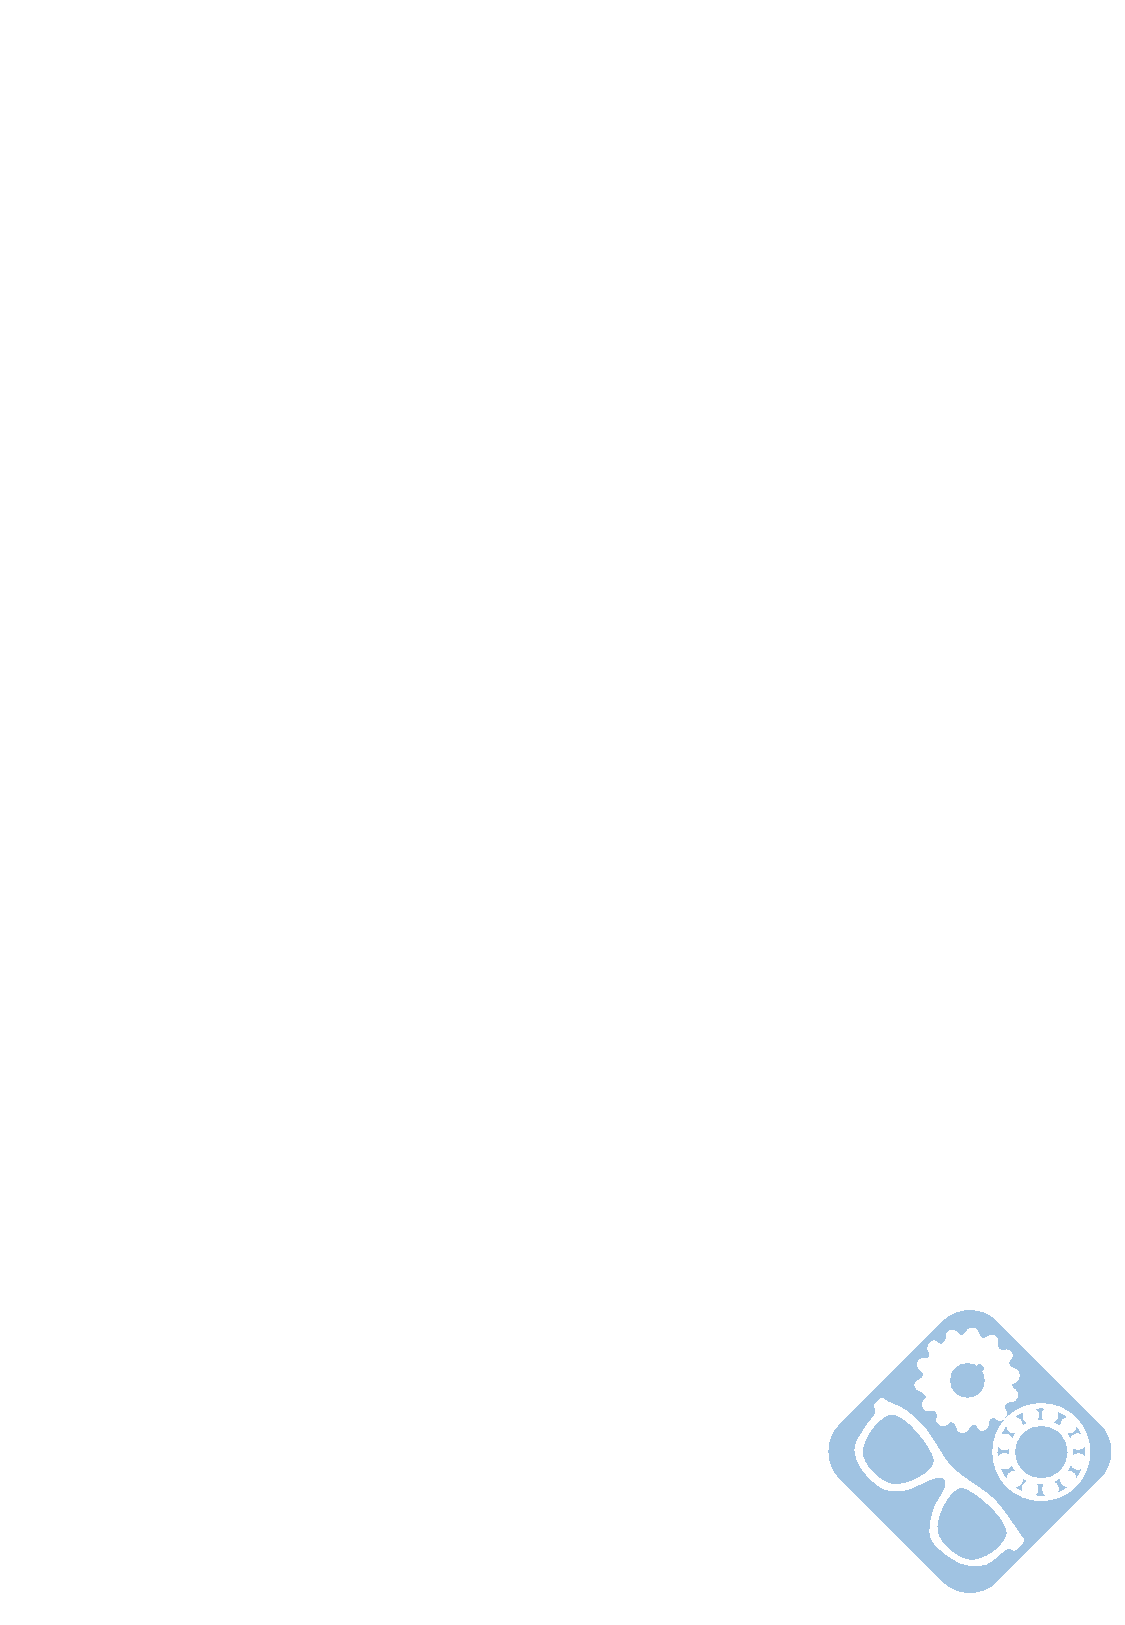
\includegraphics[width=\paperwidth,height=\paperheight,%
keepaspectratio]{../../../img/fond4}%
\end{center}
\vfill
}}}

\begin{document}

\pagestyle{empty}

\AddToShipoutPicture*{\BackgroundPic}


\includegraphics[width=2cm]{../../../img/logo}

\Huge{DS \numero - \sujet}

\vspace{1cm}

\ifdef{\prive}{\begin{center}\colorbox{danger}{\Huge{Avec Correction}}\end{center}}{}

\begin{center}
\centering\huge{PTSI}
\end{center}

\vspace{2cm}


\begin{center}
\centering\Large{\jour}
\end{center}

\vspace{2cm}

\normalsize

\tableofcontents

\newpage

\AddToShipoutPicture{\BackgroundPicdeux}

\pagestyle{fancy}

\begin{center}
\Huge \sujet
\end{center}


\normalsize


\section{Présentation du système}

\begin{figure}[ht!]
\begin{center}
 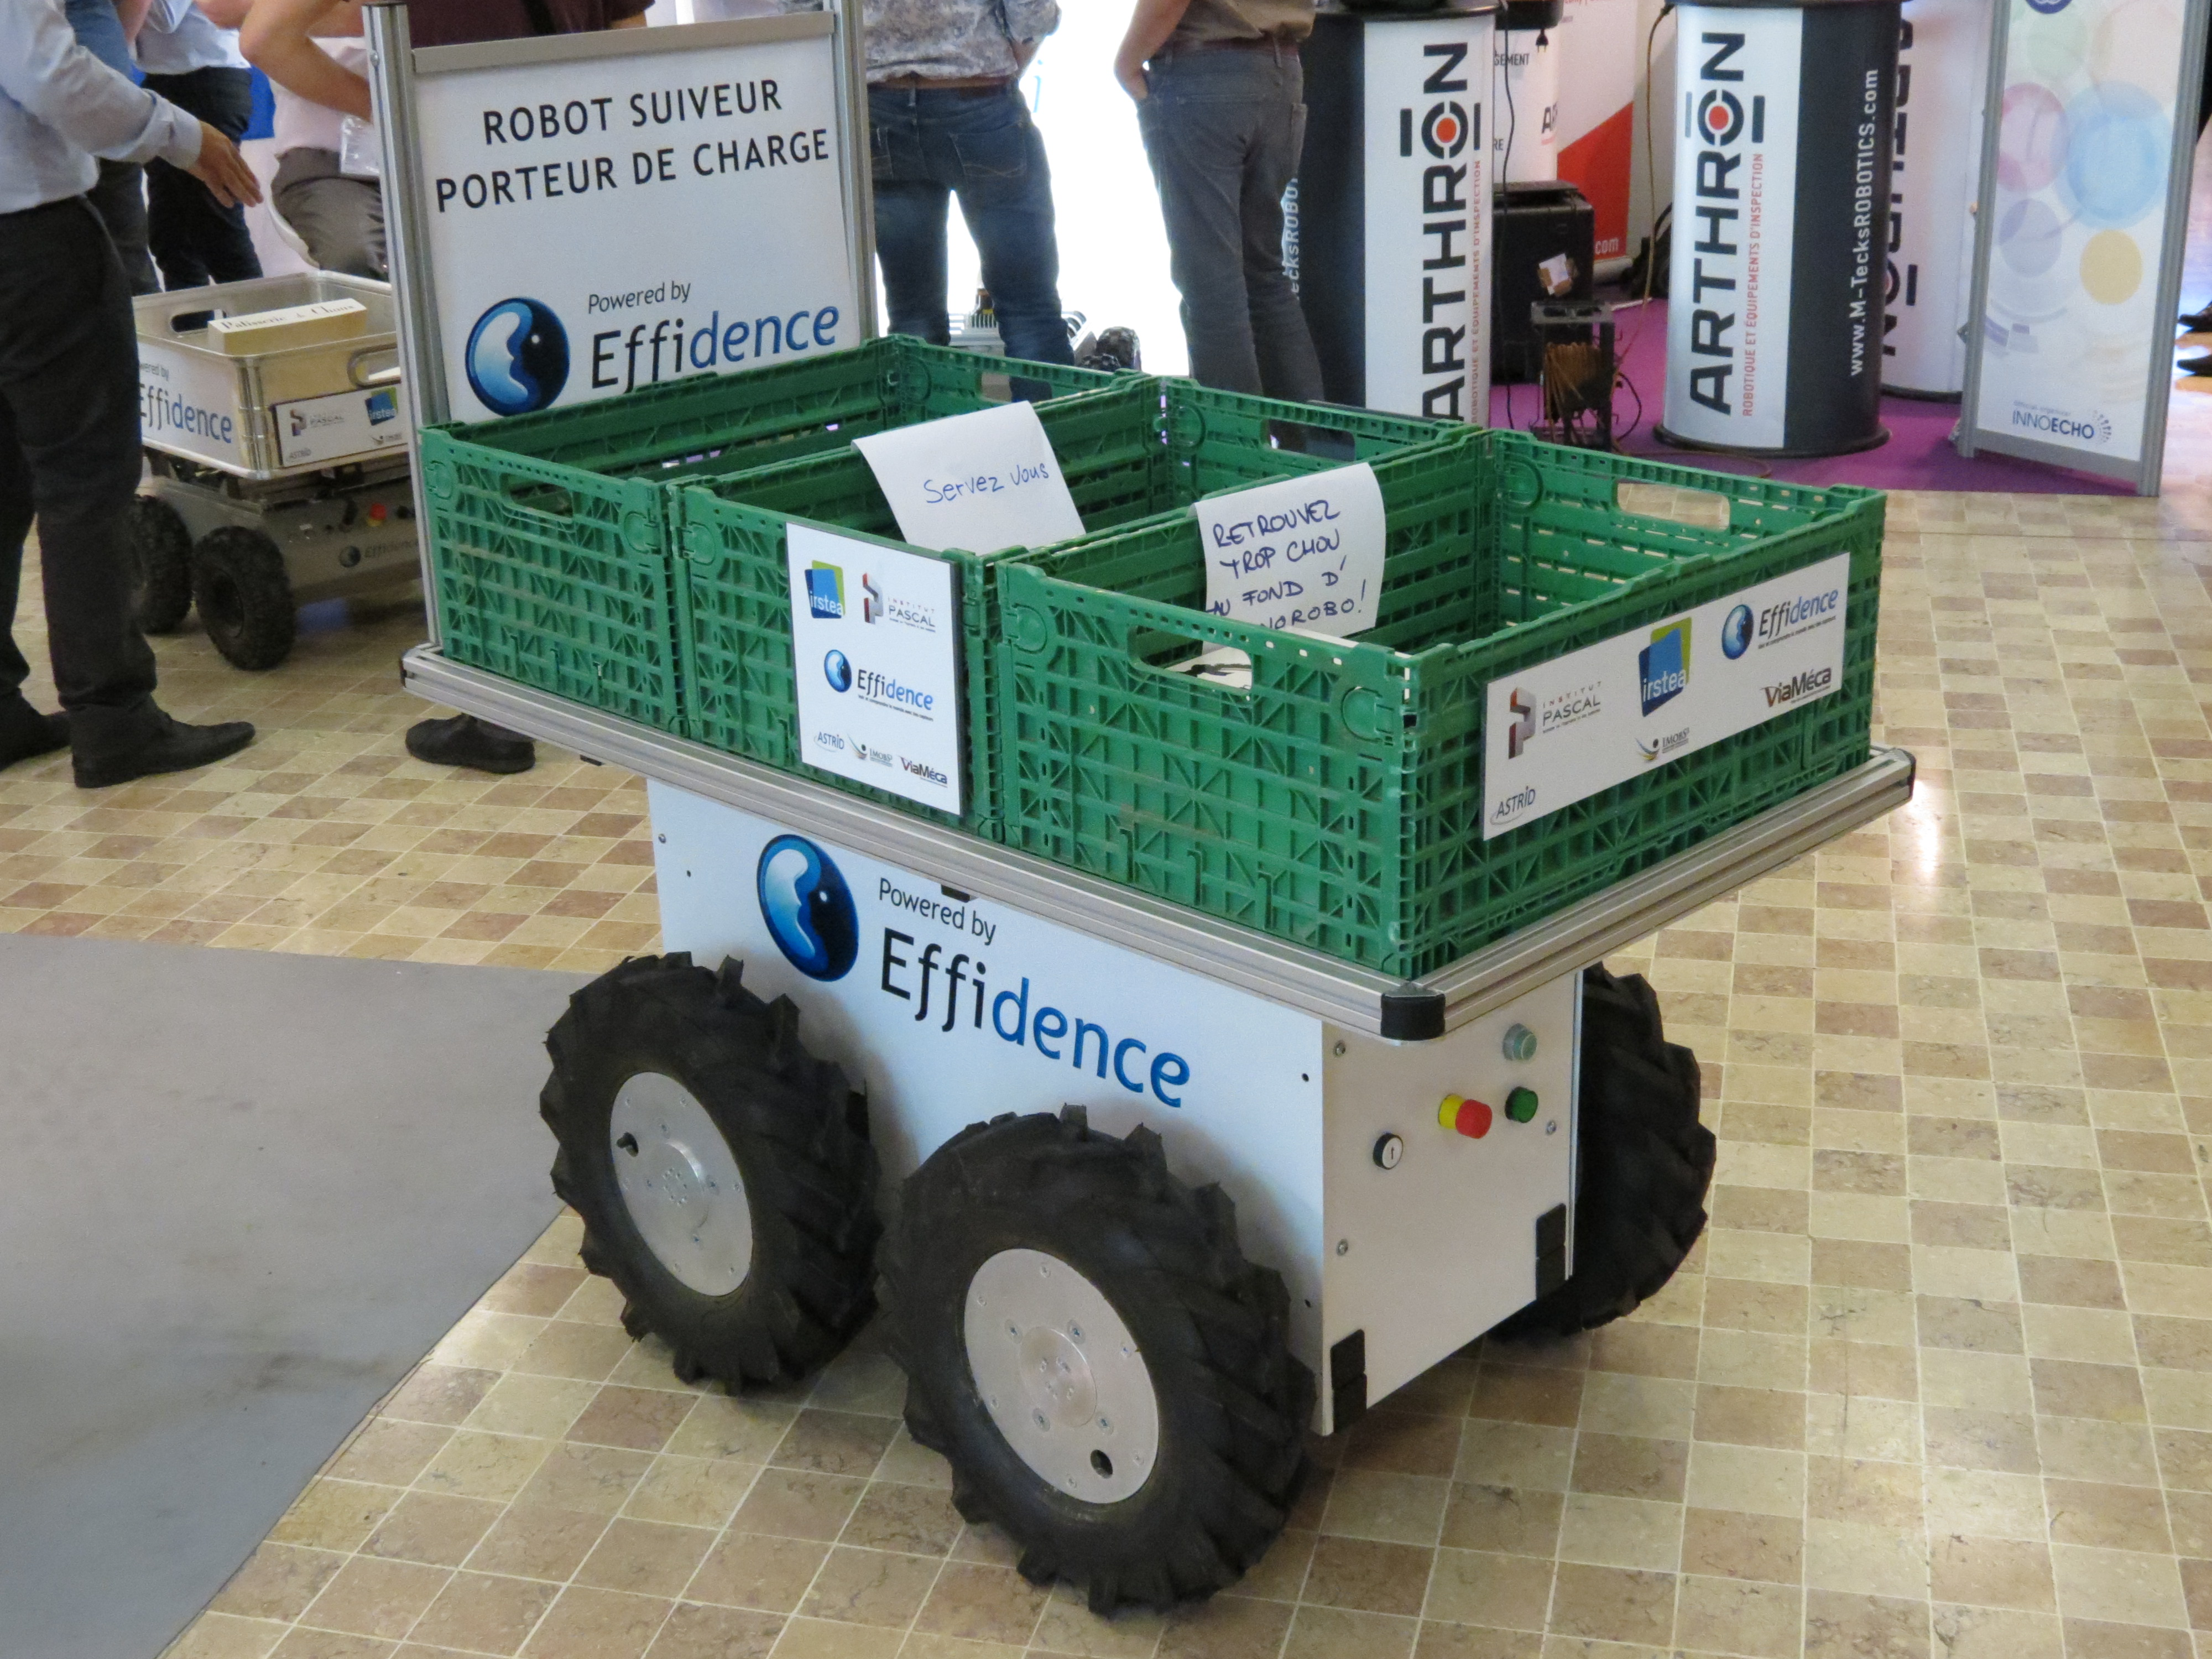
\includegraphics[width=0.6\linewidth]{img/fig01}
\end{center}
\caption{Robot \og Effibot\fg}
\label{fig01}
\end{figure}

Le sujet porte sur l'étude du robot assistant : \og Effibot \fg. Ce robot est un robot d'aide à la personne permettant de transporter des charges lourdes. Il est actuellement développé par la société française Effidence.

Cette société développe ce robot afin de répondre au plus près au besoin des utilisateurs en proposant différentes évolutions des modèles disponibles.

Le principe du fonctionnement d'\og Effibot \fg est relativement simple. L'utilisateur se place devant le robot qui le repère, à l'aide de différents capteurs et d'un traitement des informations. Le robot \og Effibot \fg suit
alors à une distance constante l'utilisateur.

Des sociétés, telles que la SNCF, travaillent en partenariat avec Effidence pour développer \og Effibot \fg afin de permettre aux usagers de transporter leurs bagages.

\begin{figure}[ht!]
\begin{center}
 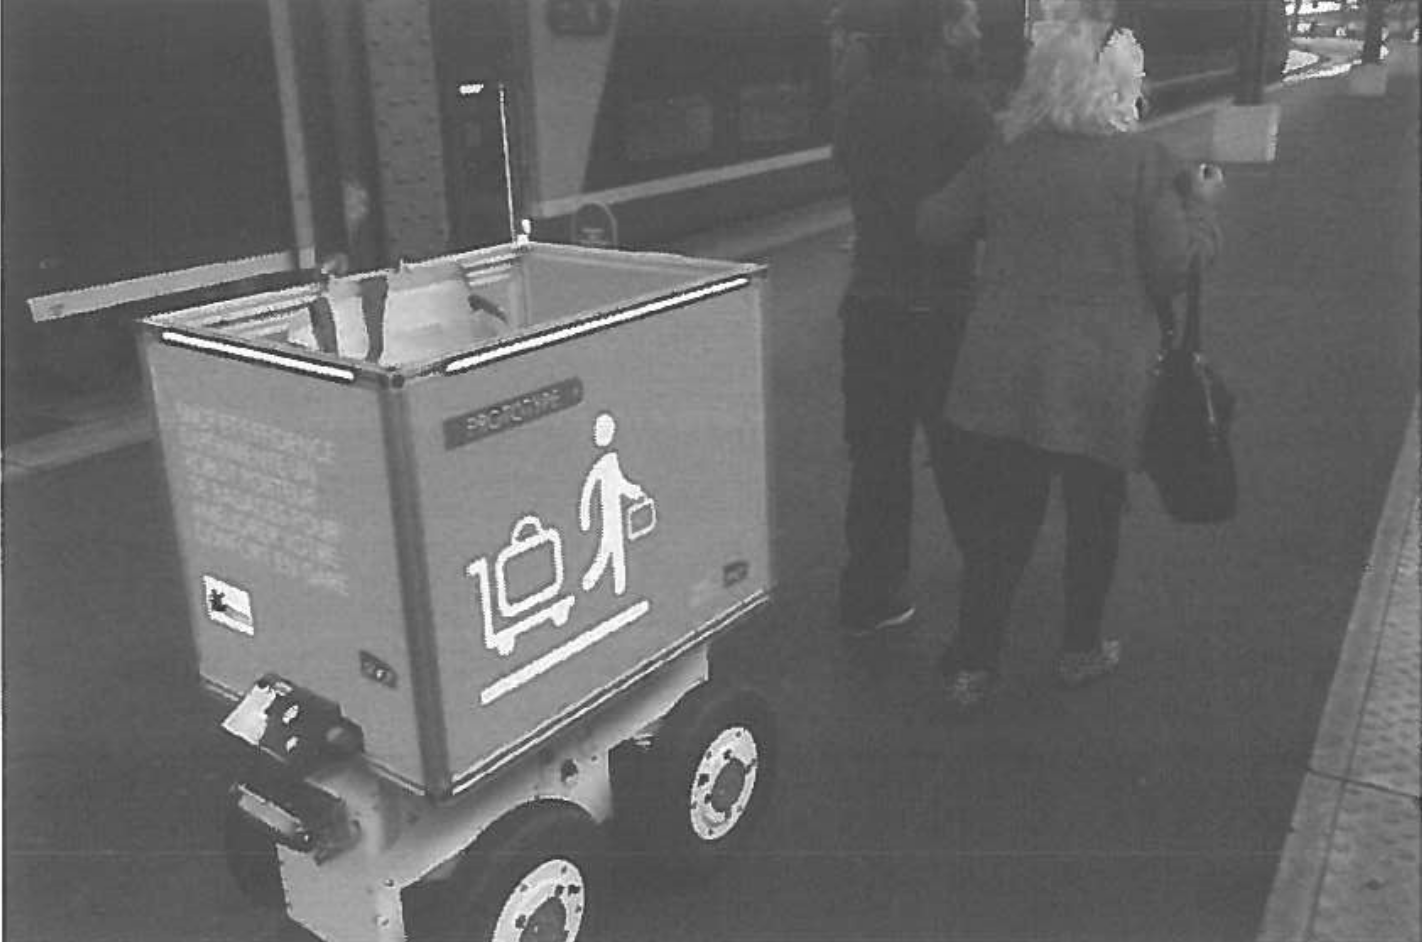
\includegraphics[width=0.6\linewidth]{img/fig02}
\end{center}
\caption{Utilisation du robot dans le transport de bagage}
\label{fig02}
\end{figure}

Ce système se développe également en partenariat avec des sociétés de BTP, de logistique ou même La Poste. Son développement se fait également à l'international avec notamment Deutsch Post (La poste allemande) pour permettre au facteur de livrer dans les villes les différents colis en réduisant la
pénibilité du transport.

D'autres domaines d'activités sont intéressés par ce robot, comme les secteurs agricole et militaire où les charges à transporter peuvent également être importantes.

\section{Présentation et plan de l'étude}

Le robot \og Effibot \fg est contrôlé par un système de commande et de navigation appelé \og Effinav \fg. Ce système de commande est le c\oe ur du savoir-faire de l'entreprise Effidence. La complexité de ce système \og Effinav \fg réside dans sa capacité à gérer plusieurs sources d'informations de différents capteurs, d'en faire une synthèse et enfin d'établir la commande des différents moteurs permettant de mouvoir le système. Afin de respecter au mieux l'exigence de suivi d'une personne, différents points vont donc être étudié dans ce sujet :

Dans une première partie, nous étudierons une modélisation de l'asservissement de suivi d'une personne dans un cas simplifié et vérifierons les performances atteintes par le système. L'étude se fera pour un suivi de personne, en ligne droite supposée parfaitement horizontale.

Dans une seconde partie, nous nous intéresserons au système de direction à quatre roues directrices de l'\og Effibot \fg. L'étude géométrique de ce système sera faite.

\section{Asservissement de suivi de personne}

Le schéma-blocs fonctionnel du système d'asservissement de suivi d'une personne est présenté sur la figure suivante. On suppose que la charge est équirépartie sur chacune des roues et que le déplacement se fait en ligne droite parfaitement horizontale.

Le déplacement de l'\og Effibot \fg est assuré par 4 roues-moteurs. Chacune des roues peut donc avoir un comportement qui lui est propre. Puisque l'étude s'effectue en ligne droite parfaitement horizontale et que la charge est équirépartie, on suppose alors un comportement équivalent pour chacune d'entre elle.

Cela nous amène a étudier l'asservissement sous cette forme :

\begin{figure}[ht!]
\begin{center}
 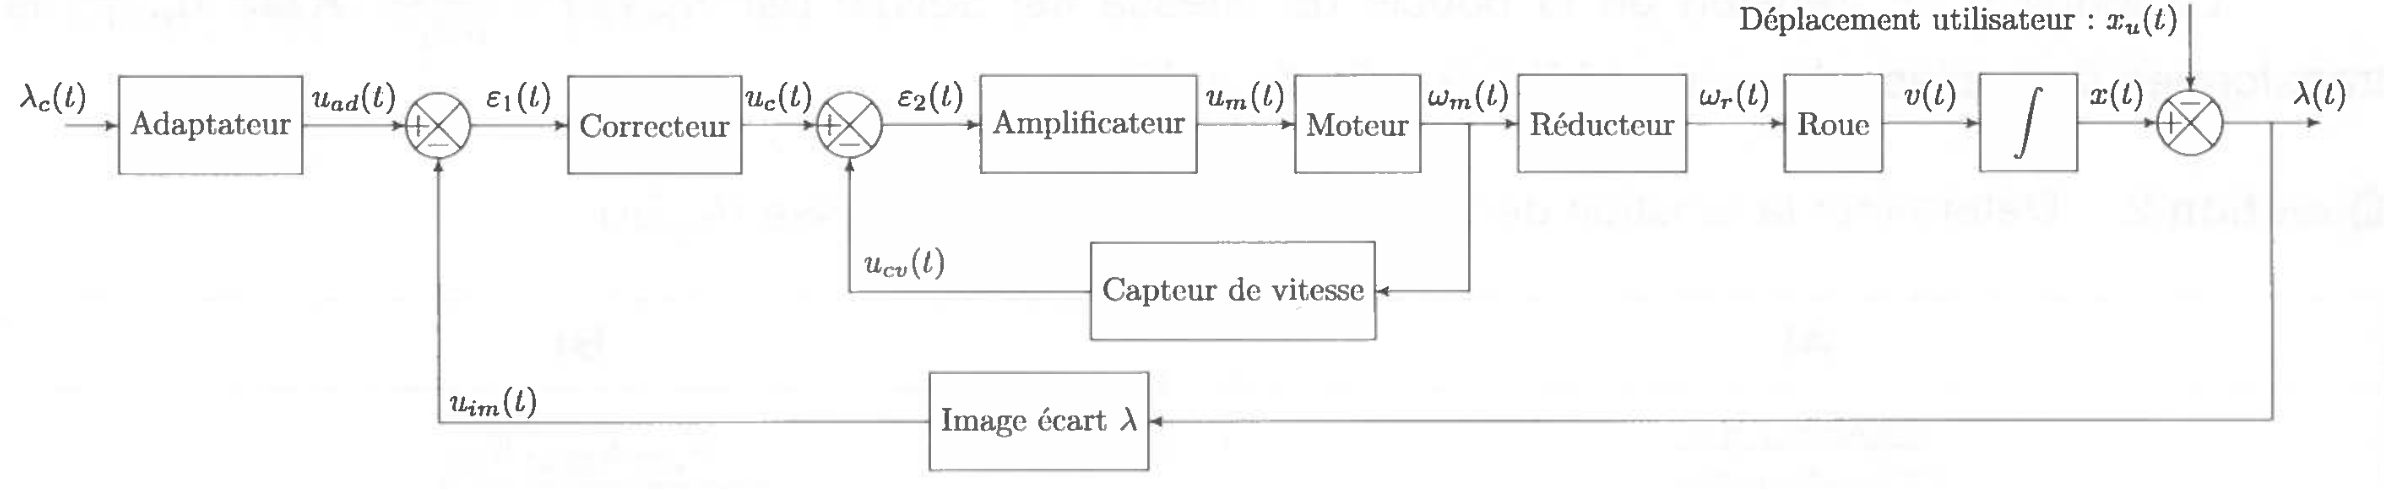
\includegraphics[width=0.9\linewidth]{img/fig03}
\end{center}
\caption{Schéma-blocs fonctionnel de l'asservissement de l'Effibot}
\label{fig03}
\end{figure}

\begin{itemize}
 \item $\lambda_c$ est la consigne d'écart (en m) que l'on veut maintenir entre l'utilisateur et l'\og Effibot \fg,
 \item $\lambda$ est la valeur d'écart (en m) entre l'utilisateur et l'\og Effibot \fg,
 \item L'adaptateur est un gain pur: $K_{ad}$ (en $V\cdot m^{-1}$) permettant d'adapter la consigne d'écart en tension de commande,
 \item Le capteur \og Image écart $\lambda$ \fg renvoie une tension image de l'écart réel entre l'utilisateur et le système, celui est modélisé par un gain pur $K_{im}$, (en $V\cdot m-^{1}$). Cette information est en réalité issue
des différents capteurs du robot et traité par le module \og Effinav \fg,
 \item L'amplificateur est modélisé par un gain pur : $K_{am}$,
 \item Le capteur de vitesse est modélisé par un gain pur : $K_{cv}$, (en $V\cdot s\cdot rad^{-1}$),
 \item Le réducteur est modélisé par un gain pur : $K_r$,
 \item La roue de l'\og Effibot \fg a un rayon $R_r$ (en $m$),
 \item Le correcteur, l'amplificateur et le moteur sont modélisés dans la suite du sujet,
 \item Le déplacement utilisateur $x_u(t)$ sera vu comme une perturbation du système.
\end{itemize}

\subsection{Modélisation des blocs}

\subsubsection{Modèle de l'adaptateur}

On souhaite pouvoir modéliser l'asservissement du système par le schéma-blocs de la figure \ref{fig04}.

\begin{figure}[ht!]
\begin{center}
 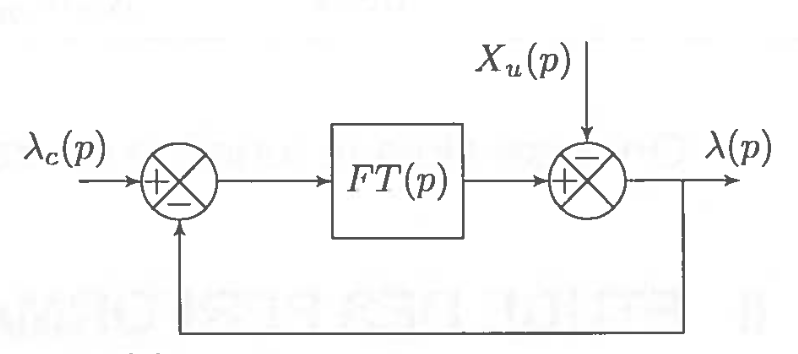
\includegraphics[width=0.3\linewidth]{img/fig04}
\end{center}
\caption{Modèle simplifié de l'asservissement}
\label{fig04}
\end{figure}

Avec $\lambda_c(p)$,$\lambda(p)$ et $X_u(p)$ les transformées de Laplace de $\lambda_c(t)$,$\lambda(t)$ et $x_u(t)$.

\question{Quelle condition doit être vérifiée par $K_{ad}$ ?}

\subsubsection{Modèle du moteur}

Le moteur permettant la mise en rotation d'une roue est un moteur brushless DC 48 V. On peut alors le modéliser par un moteur à courant continu.

La fonction de transfert du moteur peut alors se mettre sous la forme d'une fonction de transfert du second ordre de gain $K_{mot}$, de facteur d'amortissement $\xi_{mot}$ et de pulsation propre $\omega_{mot}$.

\subsubsection{Modèle de l'amplificateur de la boucle de vitesse}

La fonction de transfert de la boucle de vitesse est définie par $H_{bv}(p) = \dfrac{\Omega_m(p)}{U_c(p)}$. Avec $\Omega_m(p)$ la transformée de Laplace de $\omega(t)$ et $U_c(p)$ celle de $u_c(t)$.

\question{Déterminer la fonction de transfert de la boucle de vitesse $H_{bv}(p)$.}

\question{Déterminer l'expression de $K_{am}$ permettant d'obtenir un temps de réponse minimal de la boucle de vitesse en fonction de $\xi_{mot}$, $K_{mot}$ et $K_{cv}$.}

On pose alors la fonction de transfert de la boucle de vitesse : $H_{bv}(p)=\dfrac{K_{bv}}{1+\dfrac{2\cdot\xi_{bv}}{\omega_{bv}}\cdot p+\dfrac{p^2}{\omega_{bv}^2}}$.

\subsection{Étude des performances de l'asservissement.}

Objectif: Mettre en place une stratégie de recherche de correcteur afin de valider le cahier des charges du système.

Le cahier des charges concernant les performances de l'asservissement est donné ci-dessous :

~\

\begin{tabular}{|l|l|l|}
\hline
Exigence & Critères & Niveaux \\
\hline
Suivre un utilisateur& Précision & Erreur statique nulle, $\lambda(t\rightarrow +\infty)=\lambda_c$\\
à une distance imposée & Rapidité & $\omega_{0db}\geq 35rad.s^{-1}$ de la boucle ouverte\\
\hline
\end{tabular}

~\

%Pour rappel, dans notre étude, le déplacement de l'utilisateur $x_u(t)$ est modélisé par une rampe de pente $a$. La consigne d'écart $\lambda_c(t)$ entre l'utilisateur et l'\ogEffibot \fg est un échelon d'amplitude $\lambda_0=1m$.

D'après les différentes hypothèses et modélisations réalisées précédemment,
à l'asservissement en écart de l'\og Effibot \fg est alors le suivant :


\begin{figure}[ht!]
\begin{center}
 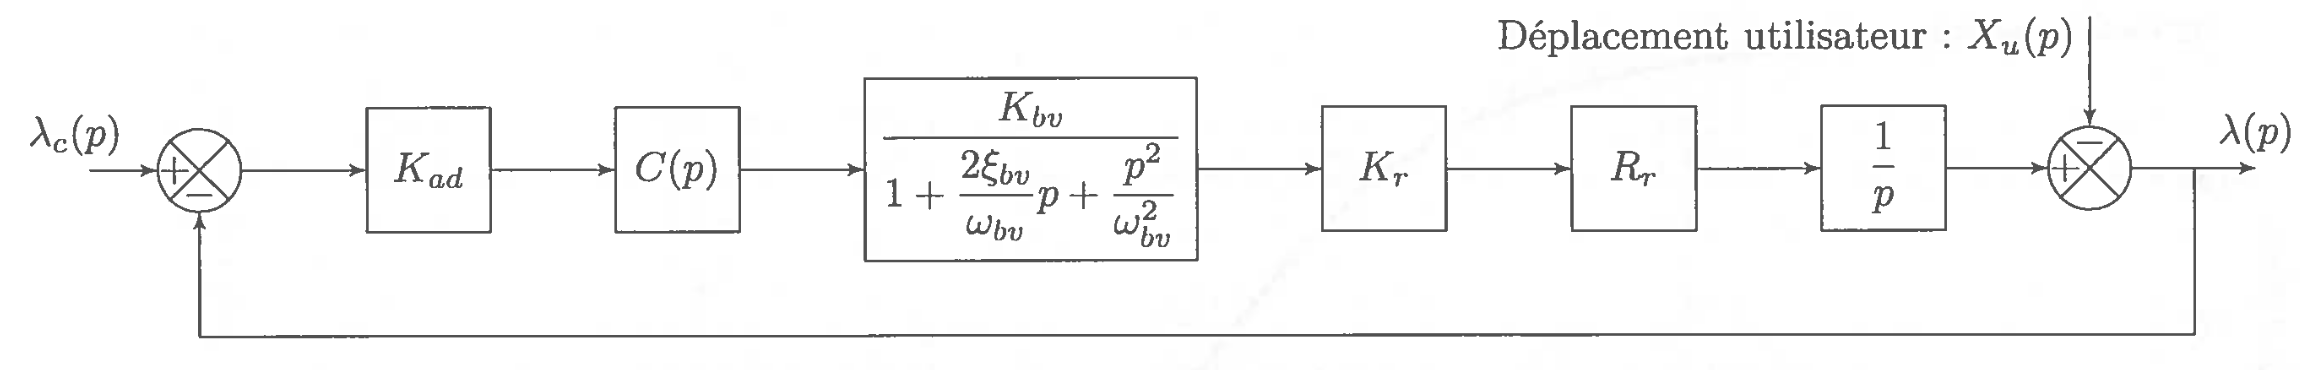
\includegraphics[width=0.9\linewidth]{img/fig05}
\end{center}
\caption{Schéma bloc de l'asservissement de l'Effibot}
\label{fig05}
\end{figure}

La perturbation sera considérée comme nulle $X_u(p)=0$. $C(p)$ est la fonction de transfert du correcteur. Dans un premier temps, on pose $C(p)=K_p$.

\question{Donner la fonction de transfert en boucle ouverte $FTBO(p)$.\label{q_FTBO}}

\subsubsection{Identification}

On cherche à identifier les caractéristiques de la fonction de transfert précédente à partir de sa réponse fréquentielle.

\begin{figure}[ht!]
\begin{center}
 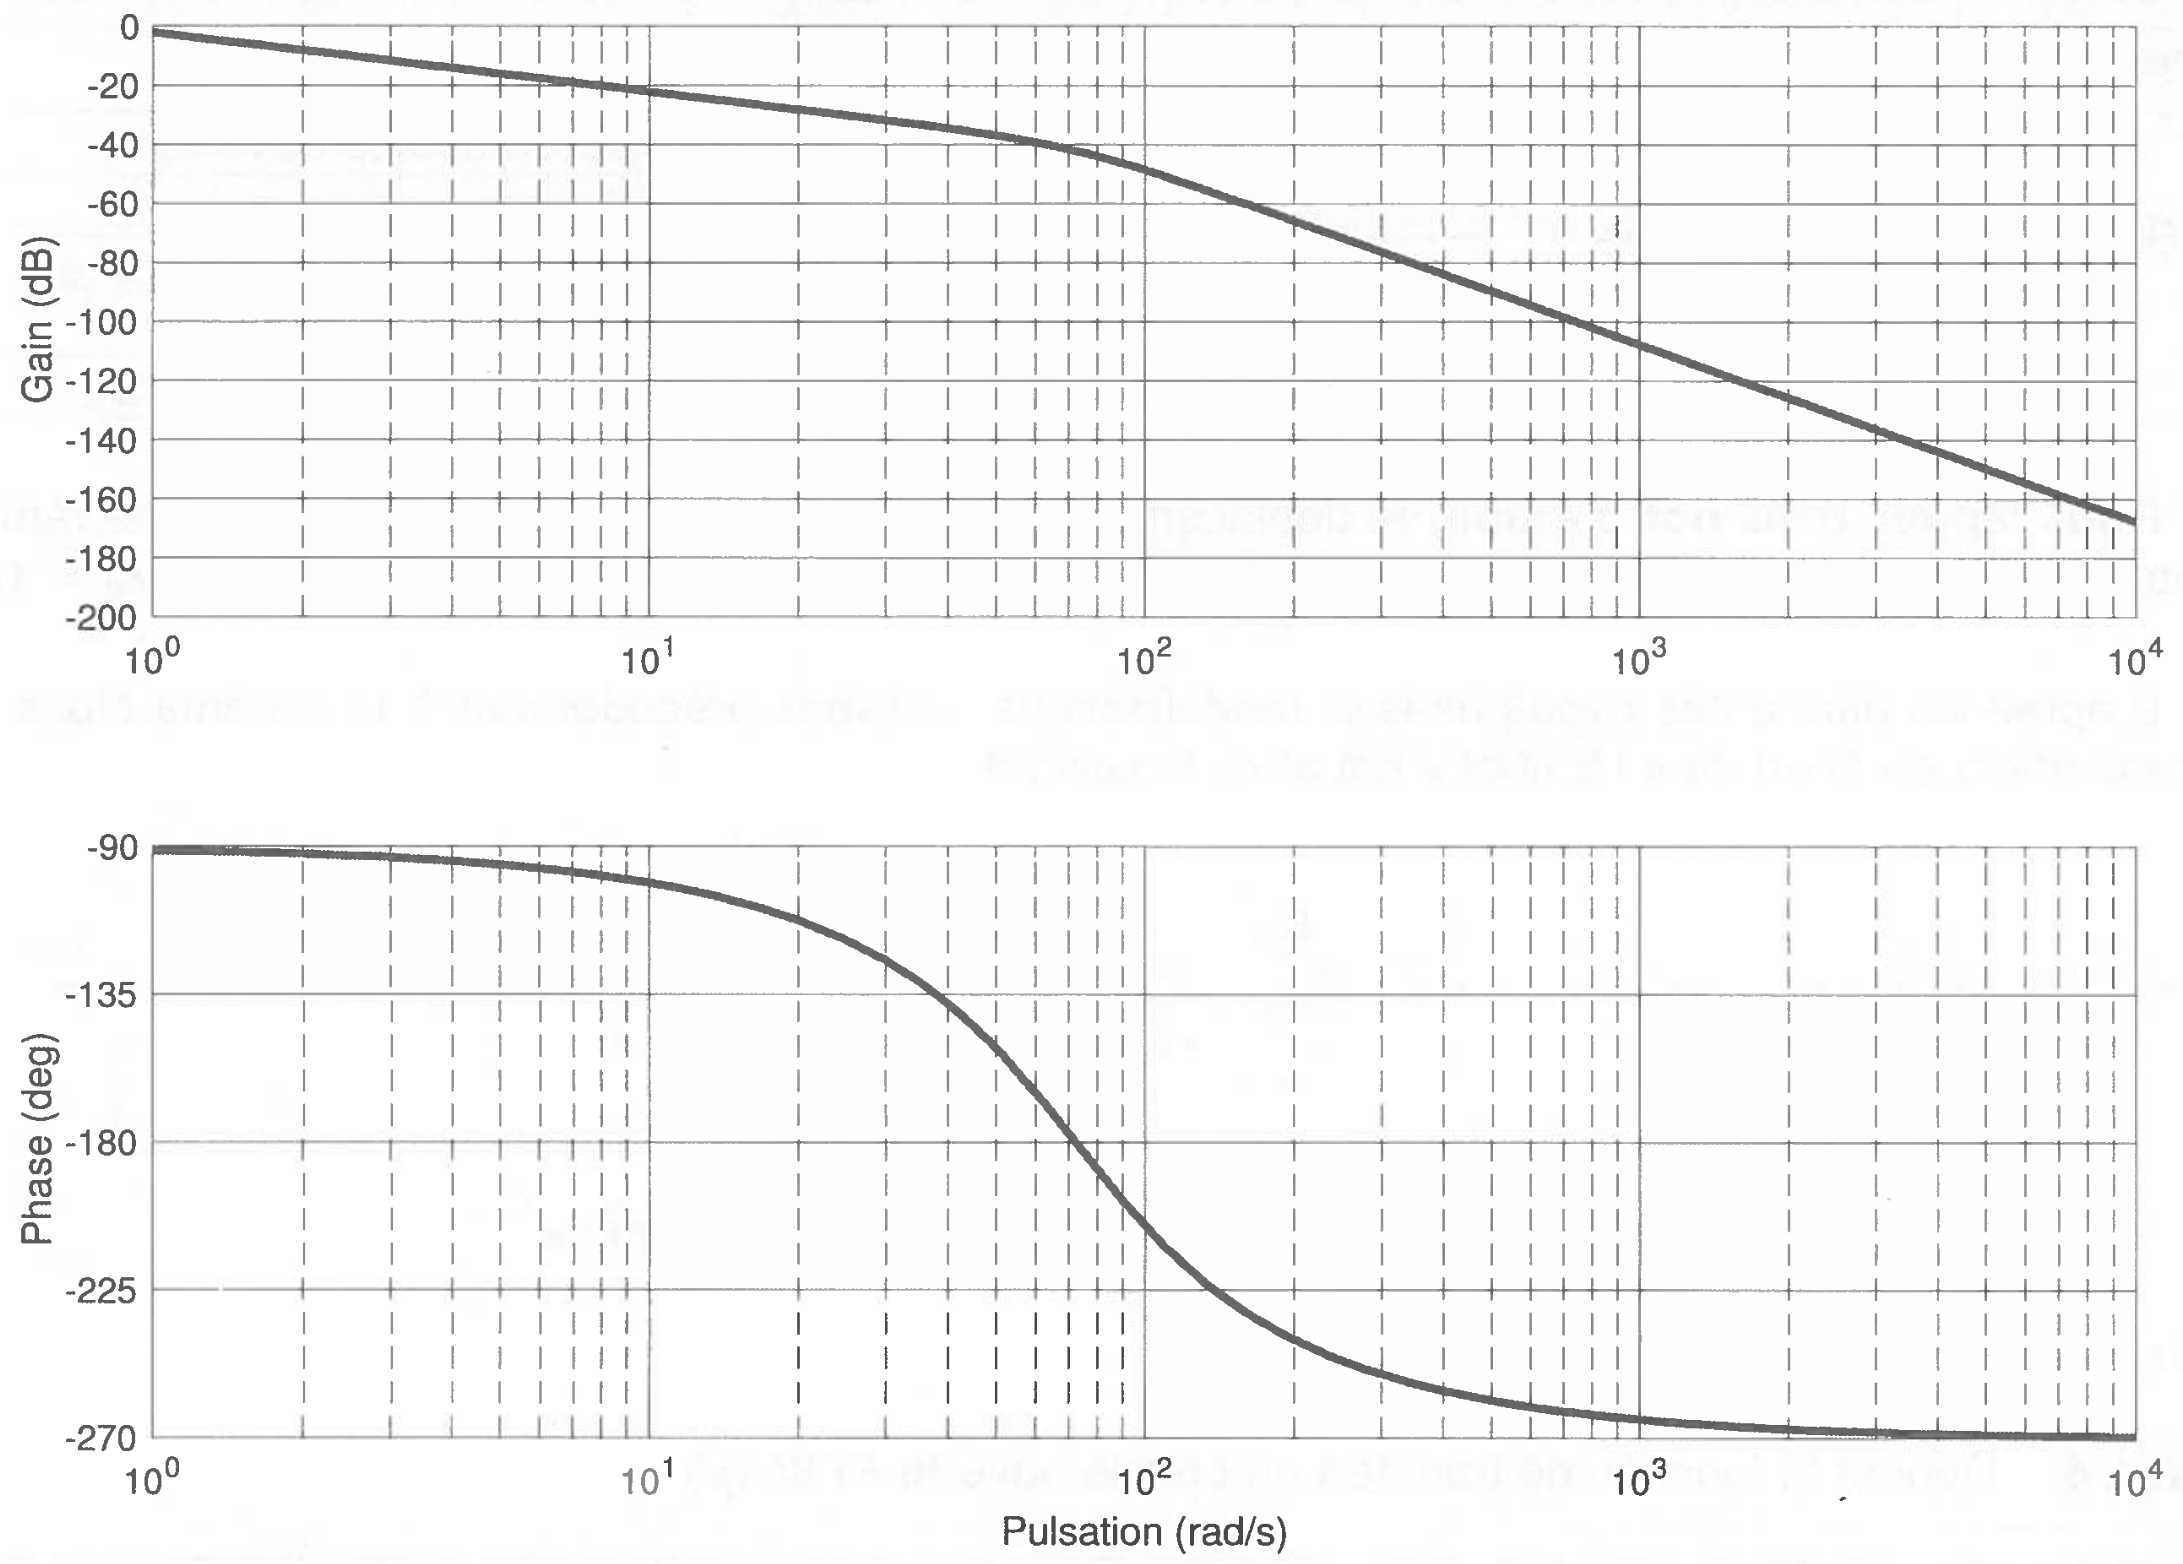
\includegraphics[width=0.8\linewidth]{img/fig06}
\end{center}
\caption{Diagramme de Bode du système en boucle ouverte}
\label{fig06}
\end{figure}

\newpage

\question{Identifier l'ordre et la classe de ce système. Cela correspond-t-il à la réponse à la question \ref{q_FTBO} ?}

\question{Déterminer les valeurs du gain de la FTBO et de la pulsation propre $\omega_{bv}$. Donner, en justifiant, une fourchette la plus précise possible pour le coefficient d'amortissement $\xi_{bv}$. \label{q_param_FTBO}}

\question{Montrer que $arg(FTBO(j\cdot\omega))=-90^\circ-arctan\left(\dfrac{\dfrac{2\cdot \xi_{bv}}{\omega_{bv}}\cdot \omega}{1-\dfrac{\omega^2}{\omega_{bv}^2}}\right)$.}

On appelle respectivement $\omega_{0dB}$ et $\omega_{-135^\circ}$ les pulsations telles que $20\cdot log\left(\left|FTBO(j\cdot\omega_{0dB})\right|\right)=0dB$ et $arg(FTBO(j\cdot\omega_{-135^\circ}))=-135^\circ$. On choisira pour la suite, $\omega_{0dB}=\omega_{-135^\circ}$.

\question{Montrer que $20\cdot log\left(\left|FTBO(j\cdot\omega_{0dB})\right|\right)=0dB$ si et seulement si $log\left(\left|\dfrac{1}{FTBO(j\cdot\omega_{0dB})}\right|\right)=0dB$.}

\question{En déduire $K_p$ en fonction de $\omega_{0dB}$, $\omega_{bv}$, $\xi_{bv}$, $K_{ad}$, $K_{bv}$, $K_{r}$ et $R_{r}$.}

\question{Déterminer $\omega_{-135^\circ}$ en fonction de $\xi_{bv}$ et $\omega_{bv}$.}

\question{A l'aide des valeurs déterminées à la question \ref{q_param_FTBO} et du résultat de la question précédente, montrer que $\xi_{bv}=1$ est une solution possible.}

\question{Cette valeur est-elle compatible avec la fourchette donnée à la question \ref{q_param_FTBO} ?}


\subsubsection{Un deuxième correcteur}

Afin d'améliorer la précision du système on se propose d'utiliser ce type de correcteur :

\begin{figure}[ht!]
\begin{center}
 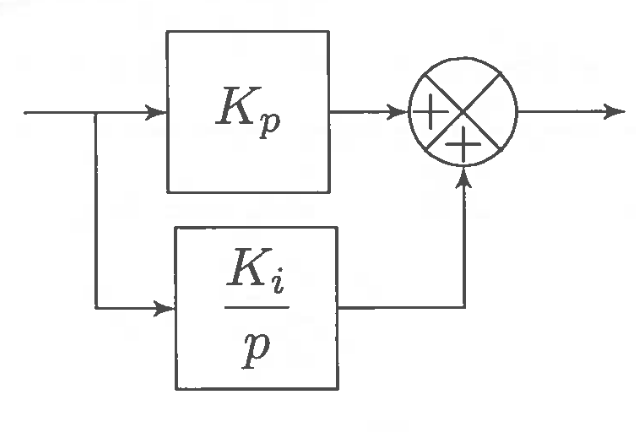
\includegraphics[width=0.3\linewidth]{img/fig07}
\end{center}
\caption{Schéma bloc du nouveau correcteur proposé}
\label{fig07}
\end{figure}

On précise que $K_p$, est le même que celui établit précédemment. On peut mettre la fonction de transfert du correcteur sous la forme : $C(p)=K_{cor}\cdot \dfrac{1+T_i\cdot p}{T_i\cdot p}$.

\question{Préciser les expressions de $K_{cor}$ et $T_i$ en fonction de $K_p$ et $K_i$.}

~\

Pour la suite, on prendra $K_{cor}=50$ et $T_i=10$.

\question{Tracer, sur le document réponse, le diagramme de Bode de la fonction $\dfrac{\dfrac{T_i}{K_{cor}}}{1+T_i\cdot p}$.}

\question{Tracer, sur le document réponse, le diagramme de Bode de la fonction $K_{cor}\cdot\dfrac{1+T_i\cdot p}{T_i}$.}

\question{Tracer, sur le document réponse, le diagramme de Bode de la fonction $C(p)$.}

\subsubsection{Analyse temporelle}

Une simulation de l'asservissement établi met en avant une tension d'alimentation du moteur brushless de $1000 V$. Ceci n'est pas physiquement viable car la tension d'alimentation maximale du moteur est limitée à $48 V$.

\question{Comment se nomme le phénomène dont il faudrait alors tenir compte dans la modélisation de la simulation établie ?}

\section{Système de direction}

\subsection{Épure de direction}

Objectif: Déterminer d'un point de vue cinématique le comportement en phase de virage, d'un véhicule a quatre roues directrices

Le système de direction de l'\og Effibot \fg s'appuie sur un système à 4 roues directrices. Ce système a pour effet d'augmenter la man\oe uvrabilité du robot lorsque celui-ci doit évoluer dans des espaces étroits.

Le principe de base est relativement simple : lorsque les roues avant braquent dans un sens, les roues arrière braquent dans l'autre sens.

\subsubsection{Détermination du rayon de courbure}

On s'intéresse ici à l'étude d'un système à 4 roues directrices avec un coefficient de proportionnalité $q$ entre les angles de braquages du train avant et du train arrière. De ce fait, si l'angle de braquage avant est de $\Phi$ celui de l'arrière est alors de $q\cdot\Phi$ avec $q\in[0,1]$.

La figure \ref{fig08} représente une épure de direction d'un système à quatre roues directrices.

Hypothèses :
\begin{itemize}
 \item $L=RF$ est la longueur d'empattement du véhicule (distance séparant les centres des trains avant et arrière),
 \item $v_a$ correspond à la voie du véhicule (largeur entre les roues)
 \item On note $F=(x_f,y_f)$ et $R=(x_r,y_r)$ les coordonnées du centre de l'essieu avant et arrière,
\item $\overrightarrow{v_f}$ et $\overrightarrow{v_r}$ correspondent respectivement à la vitesse instantanée au point $F$ et au point $R$ dans le référentiel supposé galiléen $R_0=(O_0,\overrightarrow{x_0},\overrightarrow{y_0},\overrightarrow{z_0})$,
 \item $\varphi$ caractérise l'angle que fait l'axe longitudinal du véhicule avec l'axe $\overrightarrow{x_0}$,
 \item $\Phi$ représente l'angle de braquage moyen des roues de l'essieu avant. Cet angle représente l'angle entre la direction du vecteur $\overrightarrow{v_f}$ et l'axe longitudinal,
 \item $\rho_f$ et $\rho_r$ sont les rayons de giration instantanés associés respectivement aux points $F$ et $R$,
 \item On dira ici que le rayon de courbure du virage pris par le véhicule sera égal à la distance $O_0M$, valant $\rho$,
 \item Le point $O_0$ sera considéré comme le centre du virage.
\end{itemize}

\begin{figure}[ht!]
\begin{center}
 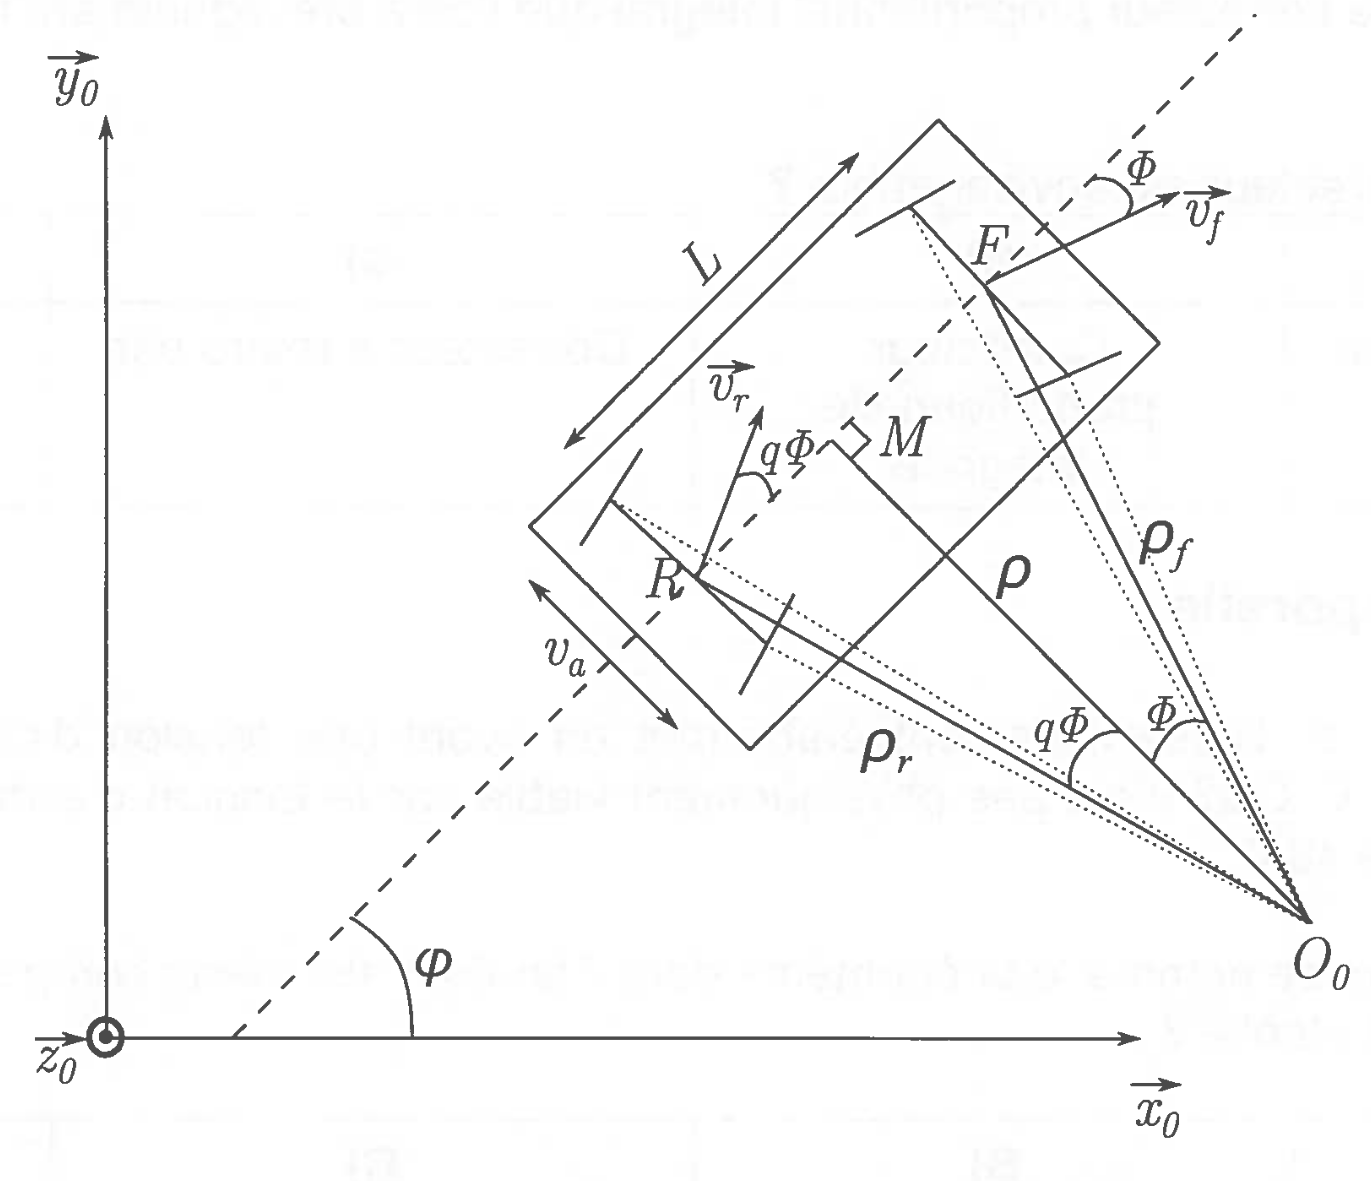
\includegraphics[width=0.6\linewidth]{img/fig09}
\end{center}
\caption{Épure de direction d'un véhicule a quatre roues directrices}
\label{fig08}
\end{figure}

\question{Quelle est la relation liant les distances $RM$ et $MF$ ?}

\question{En constatant que $RM + MF = L$, déduisez-en les expressions de $RM$ et de $MF$ en fonction de $\Phi$, $q$ et $L$.}

\question{En déduire alors l'expression de $\rho$ en fonction de $\Phi$, $q$ et $L$.}

\subsubsection{Relation angulaire idéale entre les roues}

\paragraph{Dans le reste de l'étude, on impose maintenant q=1.}

Après avoir trouvé la relation entre l'angle $\Phi$ et le rayon de courbure du virage $\rho$, on s'intéresse dans cette section à déterminer la relation théorique entre les angles de braquage des roues gauche et droite
afin d'assurer une bonne tenue de l'\og Effibot \fg en phase de virage.

Le système de direction est présenté en figure \ref{fig09}. Ce système permet une symétrie de direction entre le train avant et le train arrière. Le braquage des roues avant, gauche et droite, solidaires des fusées $3_g$, et $3_d$ est assurée via les biellettes $2_g$, et $2_d$, elles-mêmes mises en mouvement grâce à la pièce 1. La pièce 1 est mise en rotation par rapport au bâti grâce à un motoréducteur, de rapport de réduction $k_{mot}$, entraînant une roue dentée solidaire de la pièce 1. La biellette 4 assure la liaison angulaire entre le train avant et le train arrière. Les différentes figures sont présentées dans la base $B=(\overrightarrow{x},\overrightarrow{y},\overrightarrow{z})$ liée au bâti de l'\og Effibot \fg.

\begin{figure}[ht!]
\begin{center}
 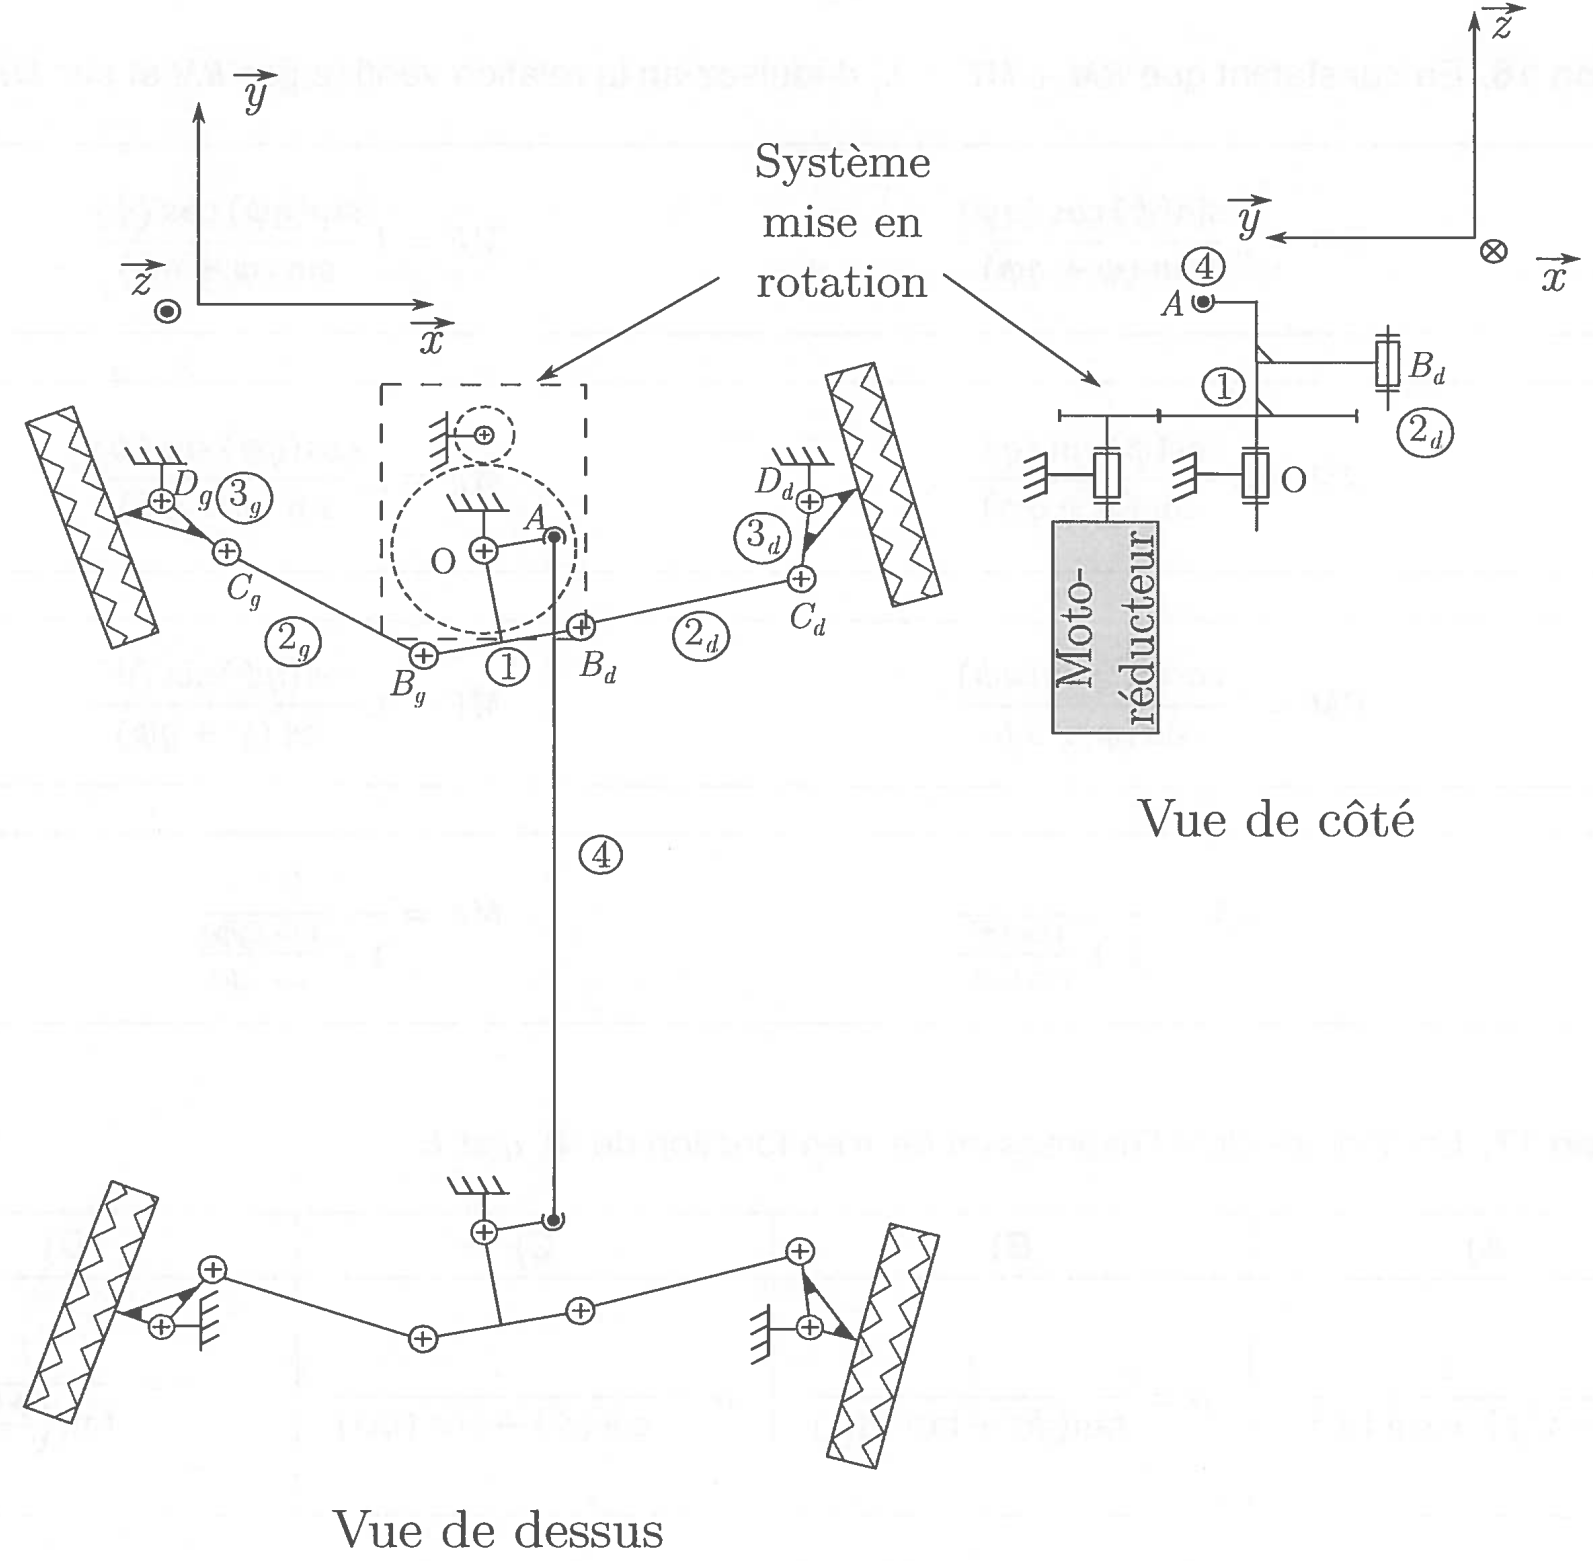
\includegraphics[width=0.6\linewidth]{img/fig10}
\end{center}
\caption{Principe du système de direction}
\label{fig09}
\end{figure}

Afin d'assurer une bonne tenue en virage, il est nécessaire que les droites perpendiculaires au plan des roues se coupent en un même point O, (voir figure \ref{fig10}).

\begin{figure}[ht!]
\begin{center}
 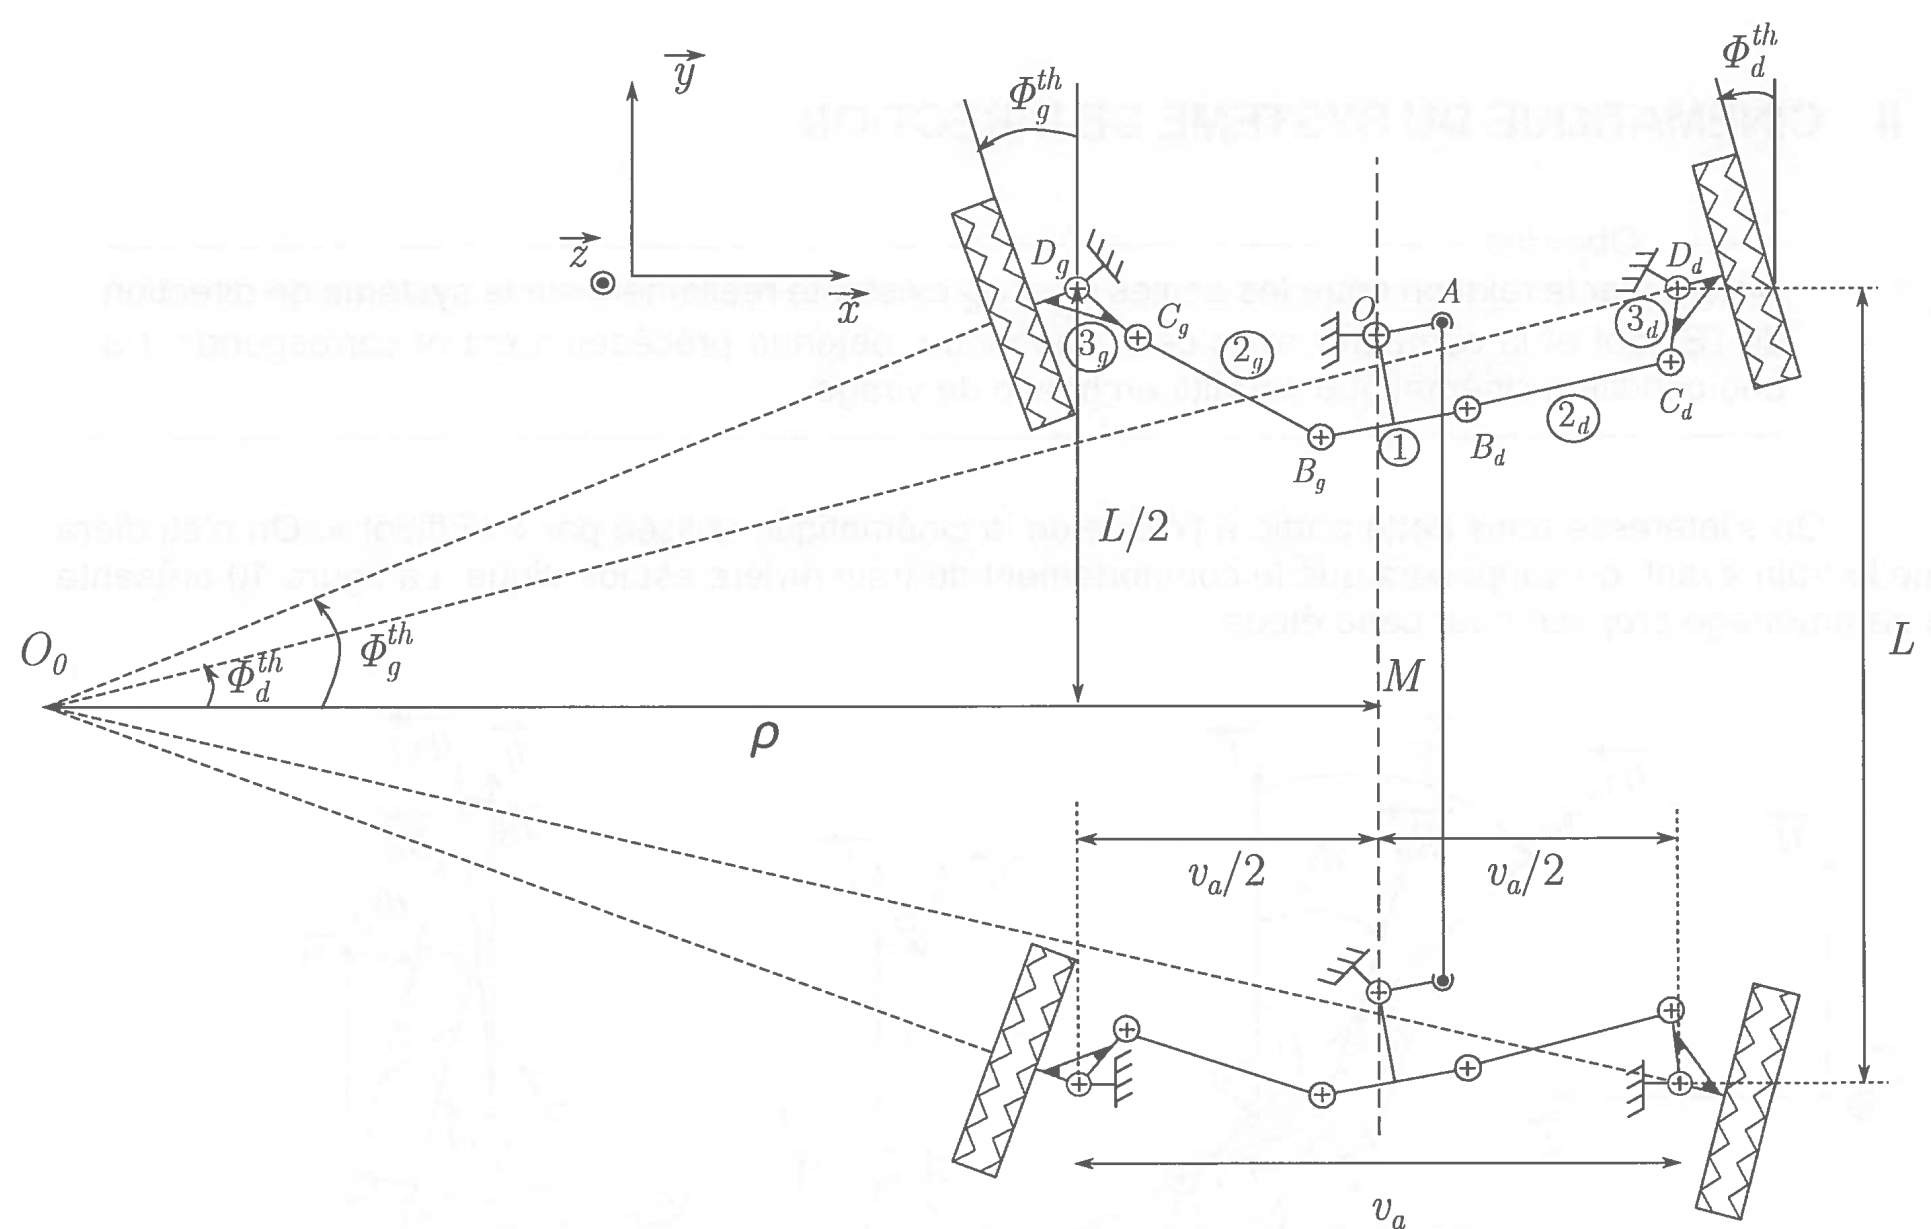
\includegraphics[width=0.8\linewidth]{img/fig11}
\end{center}
\caption{Modélisation du système de direction de l'Effibot}
\label{fig10}
\end{figure}

\newpage

\question{Déterminer la relation entre $\Phi^{th}_g$ et $\Phi^{th}_d$.}

\subsection{Cinématique du système de direction}

Objectifs: Déterminer la relation entre les angles $\Phi_g$ et $\Phi_d$ existante réellement sur le système de direction de l'Effibot et la comparer avec celle, théorique, obtenue précédemment et correspondant à une condition cinématique parfaite en phase de virage.

On s'intéresse dans cette partie à l'étude de la cinématique utilisée par \og l'Effibot \fg. On n'étudiera que le train avant, on supposera que le comportement du train arrière est identique. La figure \ref{fig12} présente le paramétrage proposé pour cette étude.

\begin{figure}[ht!]
\begin{center}
 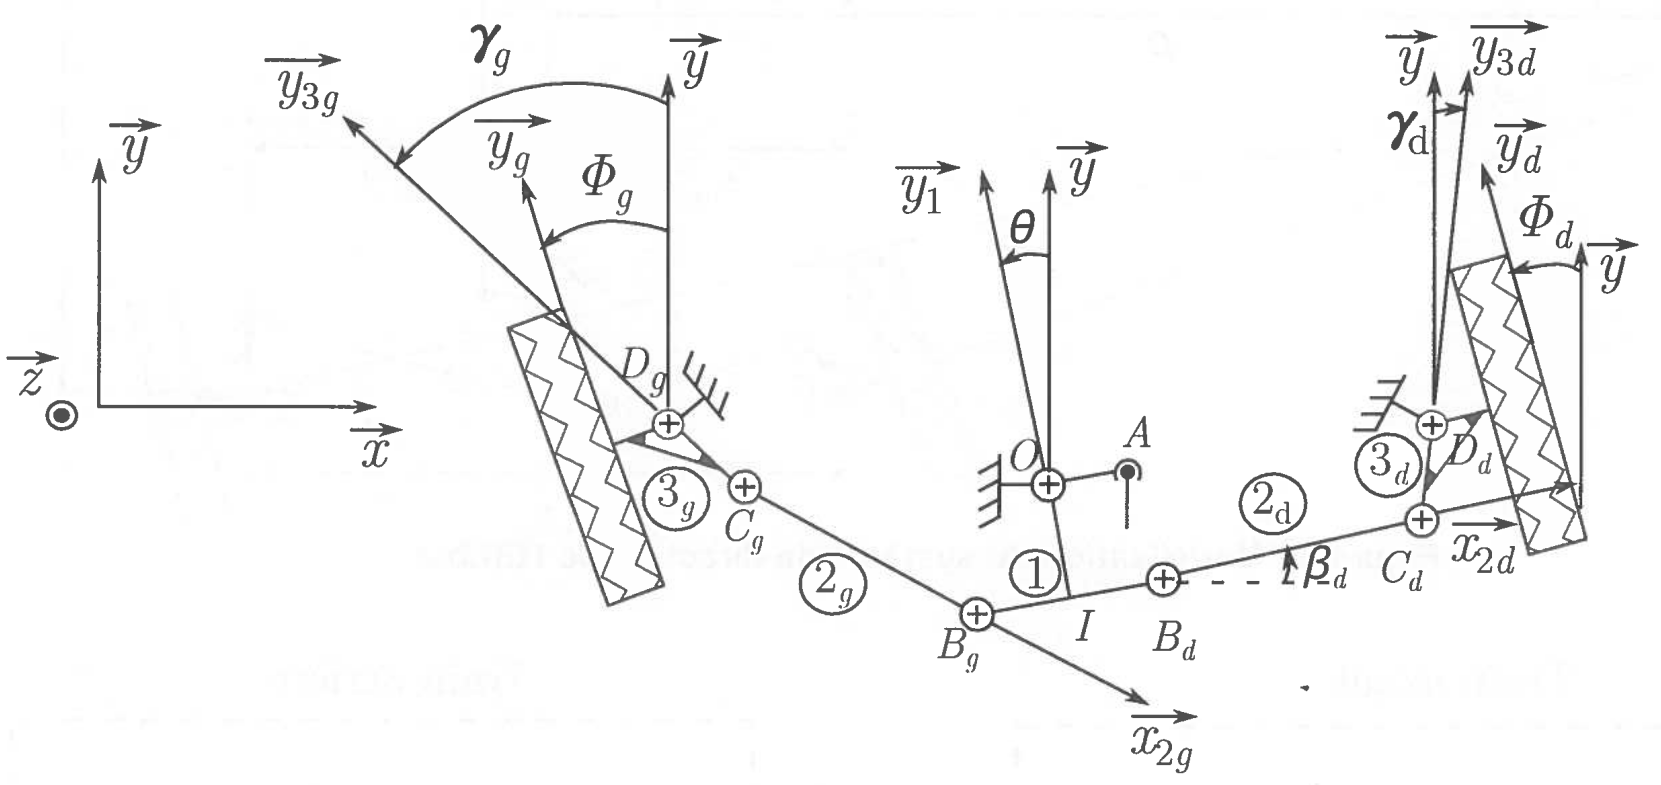
\includegraphics[width=0.6\linewidth]{img/fig12}
\end{center}
\caption{Paramétrage du système de direction}
\label{fig11}
\end{figure}

Le paramètre d'entrée est l'angle $\theta$. Les paramètres que l'on va chercher à déterminer sont les angles $\Phi_g$ et$\Phi_d$ représentatifs de l'angle de braquage des roues gauche et droite par rapport à l'axe $\overrightarrow{y}$.

On pose alors :
\begin{itemize}
 \item $(\overrightarrow{x},\overrightarrow{x_1})=(\overrightarrow{y},\overrightarrow{y_1})=\theta$,
 \item $(\overrightarrow{x},\overrightarrow{x_{2g}})=(\overrightarrow{y},\overrightarrow{y_{2g}})=\beta_g$, $(\overrightarrow{x},\overrightarrow{x_{2d}})=(\overrightarrow{y},\overrightarrow{y_{2d}})=\beta_d$,
 \item $(\overrightarrow{x},\overrightarrow{x_{3g}})=(\overrightarrow{y},\overrightarrow{y_{3g}})=\gamma_g$, $(\overrightarrow{x},\overrightarrow{x_{3d}})=(\overrightarrow{y},\overrightarrow{y_{3d}})=\gamma_d$,
 \item $(\overrightarrow{y},\overrightarrow{y_g})=\Phi_g$, $(\overrightarrow{y},\overrightarrow{y_{d}})=\Phi_d$,
 \item $\overrightarrow{y_g}$ et $\overrightarrow{y_d}$ sont des vecteurs représentant la direction de braquage des roues. En ligne droite $\overrightarrow{y_g}=\overrightarrow{y_d}\overrightarrow{y}$,
 \item $(\overrightarrow{y_{3g}},\overrightarrow{y_g})=\delta_g$ (angle constant) et $(\overrightarrow{y_{3d}},\overrightarrow{y_d})=\delta_d$ (angle constant).
\end{itemize}

On présente quelques figures géométrales (notamment celles de la partie gauche du train avant).

\begin{figure}[ht!]
\begin{center}
 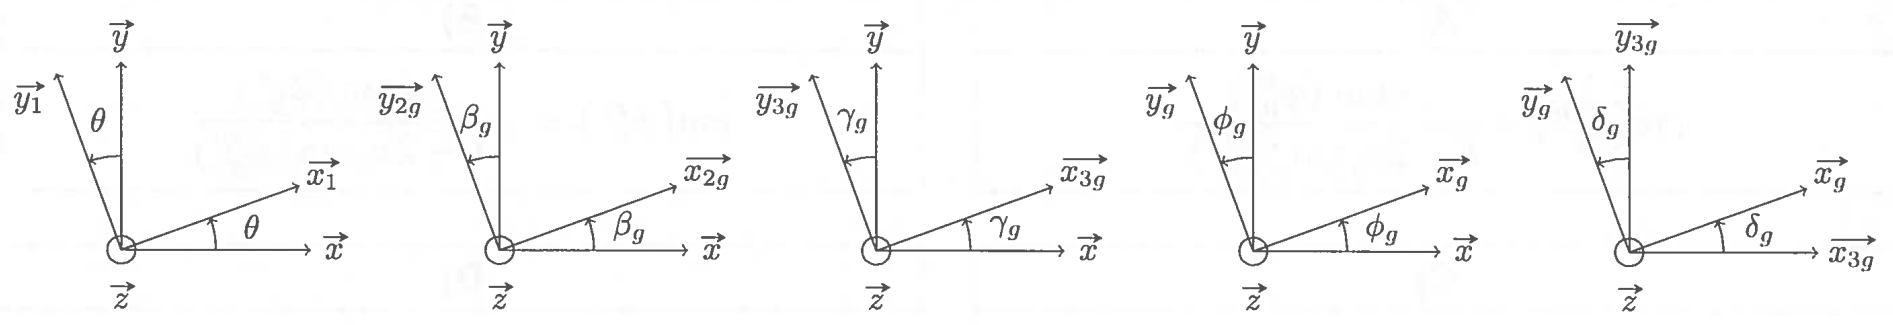
\includegraphics[width=0.9\linewidth]{img/fig13}
\end{center}
\caption{Figures de changement de repère}
\label{fig12}
\end{figure}

Les différents vecteurs de la géométrie du train avant sont donnés ci-dessous :
\begin{itemize}
 \item $\overrightarrow{OI}=-r\cdot\overrightarrow{y_1}$ (Le point O est le centre de rotation de la pièce 1 par rapport au bâti),
 \item $\overrightarrow{IB_g}=-b\cdot\overrightarrow{x_1}$,$\overrightarrow{IB_d}=b\cdot\overrightarrow{x_1}$,
 \item $\overrightarrow{B_gC_g}=-c\cdot\overrightarrow{x_{2g}}$,$\overrightarrow{B_dC_d}=c\cdot\overrightarrow{x_{2d}}$,
 \item $\overrightarrow{C_gD_g}=d\cdot\overrightarrow{y_{3g}}$,$\overrightarrow{C_dD_d}=d\cdot\overrightarrow{y_{3d}}$,
 \item $\overrightarrow{D_gO}=\dfrac{v_a}{2}\cdot\overrightarrow{x}-e\cdot\overrightarrow{y}$,
 \item $\overrightarrow{D_dO}=-\dfrac{v_a}{2}\cdot\overrightarrow{x}-e\cdot\overrightarrow{y}$
\end{itemize}

\question{Justifier l'écriture des deux équations suivantes:
\begin{eqnarray}
-r\cdot \overrightarrow{y_1}-b\cdot\overrightarrow{x_1}-c\cdot\overrightarrow{x_{2g}}+d\cdot\overrightarrow{y_{3g}}+\dfrac{v_a}{2}\cdot\overrightarrow{x}-e\cdot\overrightarrow{y}=\overrightarrow{0}\\
-r\cdot\overrightarrow{y_1}+b\cdot\overrightarrow{x_1}+c\cdot\overrightarrow{x_{2d}}+d\cdot\overrightarrow{y_{3d}}-\dfrac{v_a}{2}\cdot\overrightarrow{x}-e\cdot\overrightarrow{y}=\overrightarrow{0}
\end{eqnarray}\label{q_eq_prog}}

\question{A l'aide de la figure \ref{fig12}, déterminer les vecteurs des bases $B_1$, $B_{2g}$, $B_{2d}$, $B_{3g}$, $B_{3d}$ dans la base $B_0$.}

\question{Écrire les équations de la question \ref{q_eq_prog} dans la base $(\overrightarrow{x},\overrightarrow{y},\overrightarrow{z})$.}

\question{Après avoir projeté ces équations sur $\overrightarrow{x}$, $\overrightarrow{y}$ et $\overrightarrow{z}$ exprimer deux équations liant $\gamma_g$, $\gamma_d$, $\theta$, $r$, $b$, $c$, $d$, $e$ et $v_a$  (mais pas $\beta_g$ ni $\beta_d$).}

~\

\begin{center}
\Huge{Fin de l'épreuve}
\end{center}

\cleardoublepage

\ifdef{\public}{\pagestyle{documentreponse}}{\pagestyle{correction}}

\reponse{2}{}{$K_{ad}=K_{im}$}

\reponse{5}{}{$H_{bv}(p)=\dfrac{K_{am}\cdot H_{mot}}{1+K_{am}\cdot H_{mot}\cdot K_{cv}}=\dfrac{\dfrac{K_{am}\cdot H_{mot}}{1+K_{am}\cdot K_{mot}\cdot K_{cv}}}{1+\dfrac{2\cdot\xi_{mot}\cdot p}{\omega_{mot}\cdot(1+K_{am}\cdot K_{mot}\cdot K_{cv})}+\dfrac{p^2}{\omega^2_{mot}\cdot(1+K_{am}\cdot K_{mot}\cdot K_{cv})}}$
}

\reponse{5}{}{$T_{R5\%}$ est minimal si $\xi_{bv}=0.69$

$\omega_{bv}=\omega_{mot}\cdot\sqrt{1+K_{am}\cdot K_{mot}\cdot K_{cv}}$

$\dfrac{2\cdot\xi_{mot}}{\omega_{mot}\cdot(1+K_{am}\cdot K_{mot}\cdot K_{cv})}=\dfrac{2\cdot \xi_{bv}}{\omega_{bv}}=\dfrac{2\cdot 0.69}{\omega_{mot}\cdot\sqrt{1+K_{am}\cdot K_{mot}\cdot K_{cv}}}$

$\dfrac{\xi_{mot}}{0.69}=\sqrt{1+K_{am}\cdot K_{mot}\cdot K_{cv}}$

$\left(\dfrac{\xi_{mot}}{0.69}\right)^2-1=K_{am}\cdot K_{mot}\cdot K_{cv}$

$K_{am}=\left[\left(\dfrac{\xi_{mot}}{0.69}\right)^2-1\right]\cdot\dfrac{1}{K_{mot}\cdot K_{cv}}$
}

\reponse{4}{}{
$FTBO(p)=\dfrac{C(p)\cdot K_{ad}\cdot K_{bv} \cdot K_r\cdot R_r}{\left(1+\dfrac{2\cdot \xi_{bv}}{\omega_{bv}}\cdot p+\dfrac{p^2}{\omega^2_{bv}}\right)\cdot p}$}

\reponse{2}{}{Il s'agit d'un système de classe 1 et d'ordre 3.}

\reponse{4}{}{Par lecture $\omega_{bv}=100rad.s^{-1}$, $K=1$ (lecture en $\omega=1rad.s^{-1}$. Il n'y a pas de résonance et pas 2 cassures, donc $\dfrac{\sqrt{2}}{2}<\xi_{bv}<2$ }

\reponse{5}{}{
 $arg(FTBO(j\cdot\omega))=arg\left(\dfrac{C(p)\cdot K_{ad}\cdot K_{bv} \cdot K_r\cdot R_r}{\left(1+\dfrac{2\cdot \xi_{bv}}{\omega_{bv}}\cdot p-\dfrac{\omega^2}{\omega^2_{bv}}\right)\cdot p}\right)= -arg\left(\dfrac{1+\dfrac{2\cdot \xi_{bv}}{\omega_{bv}}\cdot j\cdot\omega-\dfrac{\omega^2}{\omega^2_{bv}}}{K_p\cdot K_{ad}\cdot K_{bv} \cdot K_r\cdot R_r}\right)-arg(j\cdot\omega)=-90^\circ-arctan\left(\dfrac{\dfrac{2\cdot \xi_{bv}}{\omega_{bv}}\cdot \omega}{1-\dfrac{\omega^2}{\omega_{bv}^2}}\right)$
}

\reponse{5}{}{
$20\cdot log\left(\left|FTBO(j\cdot\omega_{0dB})\right|\right)=0dB$ si et seulement si $log\left(\left|FTBO(j\cdot\omega_{0dB})\right|\right)=0dB$
si et seulement si $-log\left(\left|\dfrac{1}{FTBO(j\cdot\omega_{0dB})}\right|\right)=0dB$
}

\reponse{7}{}{
$\dfrac{1}{FTBO(p)}=\dfrac{\left(1+\dfrac{2\cdot \xi_{bv}}{\omega_{bv}}\cdot p+\dfrac{p^2}{\omega^2_{bv}}\right)\cdot p}{K_p\cdot K_{ad}\cdot K_{bv} \cdot K_r\cdot R_r}=\dfrac{\left(\left(1-\dfrac{\omega^2}{\omega^2_{bv}}\right)+j\cdot \dfrac{2\cdot \xi_{bv}\cdot \omega}{\omega_{bv}}\right)\cdot j\cdot \omega}{K_p\cdot K_{ad}\cdot K_{bv} \cdot K_r\cdot R_r}$

$\left|\dfrac{1}{FTBO(p)}\right|=\dfrac{\sqrt{\left(1-\dfrac{\omega^2}{\omega^2_{bv}}\right)^2+\cdot \dfrac{4\cdot \xi^2_{bv}\cdot \omega^2}{\omega^2_{bv}}}\cdot \omega}{K_p\cdot K_{ad}\cdot K_{bv} \cdot K_r\cdot R_r}$

$20\cdot log\left(\left|FTBO(j\cdot\omega_{0dB})\right|\right)=0dB$ si et seulement si 
$\left|\dfrac{1}{FTBO(j\cdot\omega_{0dB})}\right|=1$, donc


$K_p=\dfrac{\sqrt{\left(1-\dfrac{\omega^2_{0dB}}{\omega^2_{bv}}\right)^2+\cdot \dfrac{4\cdot \xi^2_{bv}\cdot \omega_{0dB}^2}{\omega^2_{bv}}}\cdot \omega_{0dB}}{K_{ad}\cdot K_{bv} \cdot K_r\cdot R_r}$}

\reponse{7}{}{
$-90^\circ-arctan\left(\dfrac{\dfrac{2\cdot \xi_{bv}}{\omega_{bv}}\cdot \omega_{-135^\circ}}{1-\dfrac{\omega_{-135^\circ}^2}{\omega_{bv}^2}}\right)=-135$

$arctan\left(\dfrac{\dfrac{2\cdot \xi_{bv}}{\omega_{bv}}\cdot \omega_{-135^\circ}}{1-\dfrac{\omega_{-135^\circ}^2}{\omega_{bv}^2}}\right)=45$

$\dfrac{\dfrac{2\cdot \xi_{bv}}{\omega_{bv}}\cdot \omega_{-135^\circ}}{1-\dfrac{\omega_{-135^\circ}^2}{\omega_{bv}^2}}=1$

$\dfrac{2\cdot \xi_{bv}}{\omega_{bv}}\cdot \omega_{-135^\circ}=1-\dfrac{\omega_{-135^\circ}^2}{\omega_{bv}^2}$

$\dfrac{2\cdot \xi_{bv}}{\omega_{bv}}\cdot \omega_{-135^\circ}=1-\dfrac{\omega_{-135^\circ}^2}{\omega_{bv}^2}$

$\omega_{-135^\circ}^2+2\cdot \xi_{bv}\cdot\omega_{bv}\cdot \omega_{-135^\circ}-\omega_{bv}^2=0$

$\Delta=4\cdot \xi^2_{bv}\cdot\omega^2_{bv}+4\cdot\omega_{bv}^2=4\cdot\omega_{bv}^2\cdot(\xi^2_{bv}+1)$

$\omega_{-135^\circ}=\omega_{bv}\cdot(\sqrt{\xi^2_{bv}+1}-\xi_{bv})$
}

\reponse{3}{}{On détermine graphiquement $\omega_{-135^\circ}=40rad.s^{-1}$ et on avait montré que $\omega_{bv}=100rad.s^{-1}$

Donc $\omega_{bv}\cdot(\sqrt{\xi^2_{bv}+1}-\xi_{bv})=100\cdot(\sqrt{1+1}-1)=100\cdot 0.4=40$, cela correspond bien.}

\ifdef{\public}{\newpage}{}

\reponse{2}{}{Cette valeur est compatible avec la fourchette déterminée précédemment.}

\reponse{6}{}{$H_{cor(p)}=K_p+\dfrac{K_i}{p}=\dfrac{K_p\cdot p+K_i}{p}=\dfrac{1+\dfrac{K_p}{K_i}\cdot p}{\dfrac{1}{K_i}p}=K_p\cdot\dfrac{1+\dfrac{K_p}{K_i}\cdot p}{\dfrac{K_p}{K_i}p}$

Donc, $K_{cor}=K_p$ et $T_i=\dfrac{K_p}{K_i}$}

\reponse{0}{\begin{center}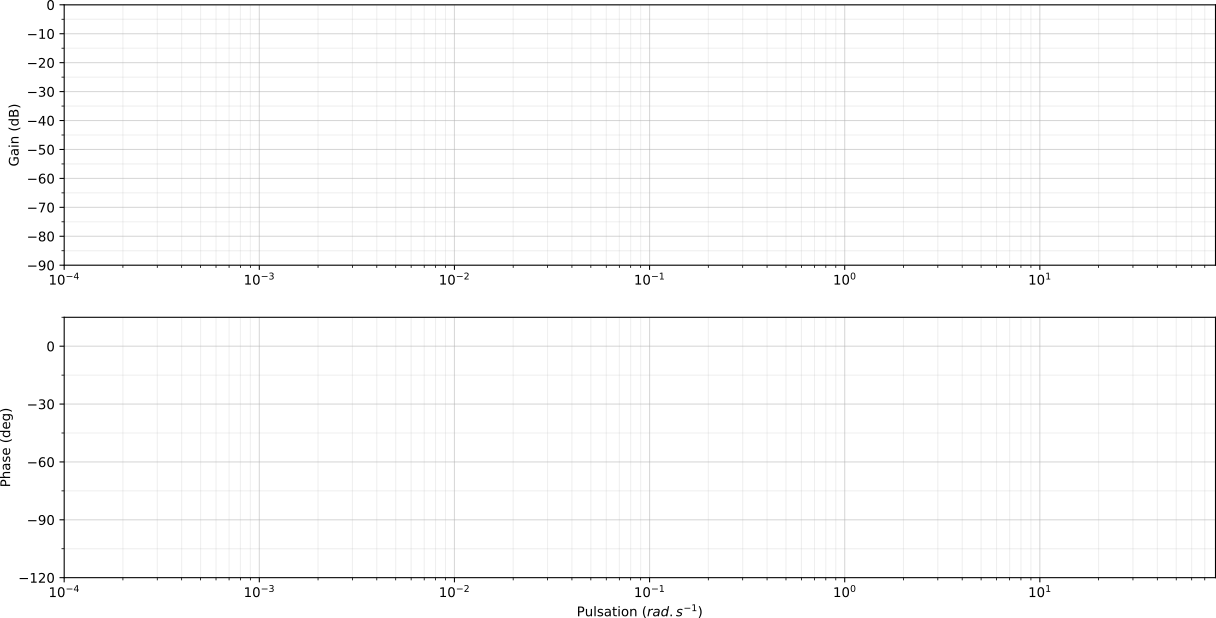
\includegraphics[width=\linewidth]{img/Bode_1}
\end{center}}{\begin{center}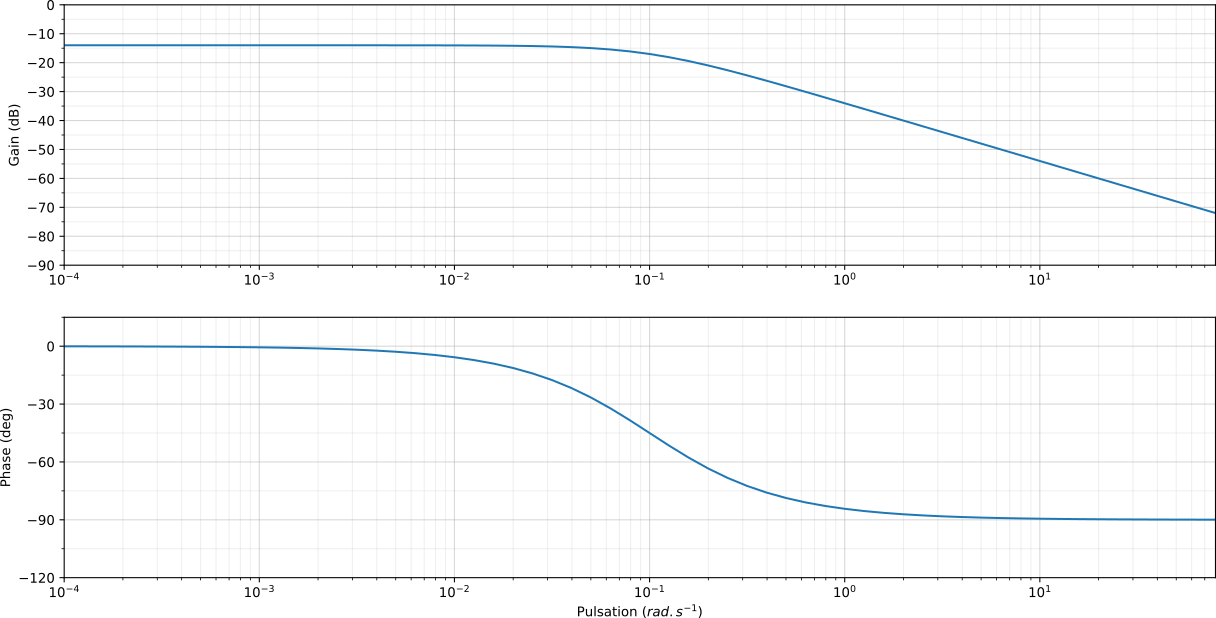
\includegraphics[width=\linewidth]{img/Bode_1_cor}
\end{center}}

\reponse{0}{\begin{center}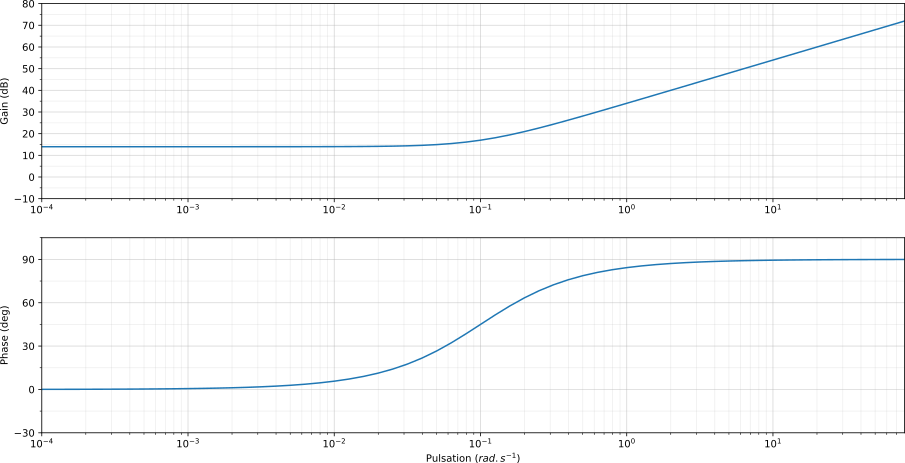
\includegraphics[width=\linewidth]{img/Bode_2}
\end{center}}{\begin{center}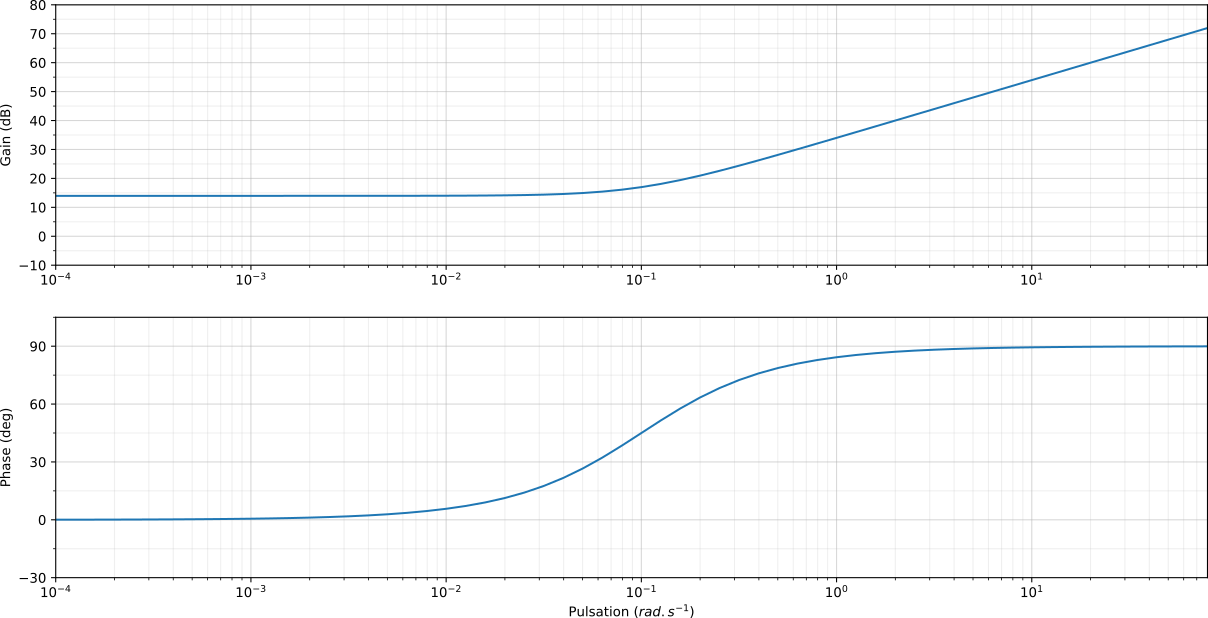
\includegraphics[width=\linewidth]{img/Bode_2_cor}
\end{center}}

\reponse{0}{\begin{center}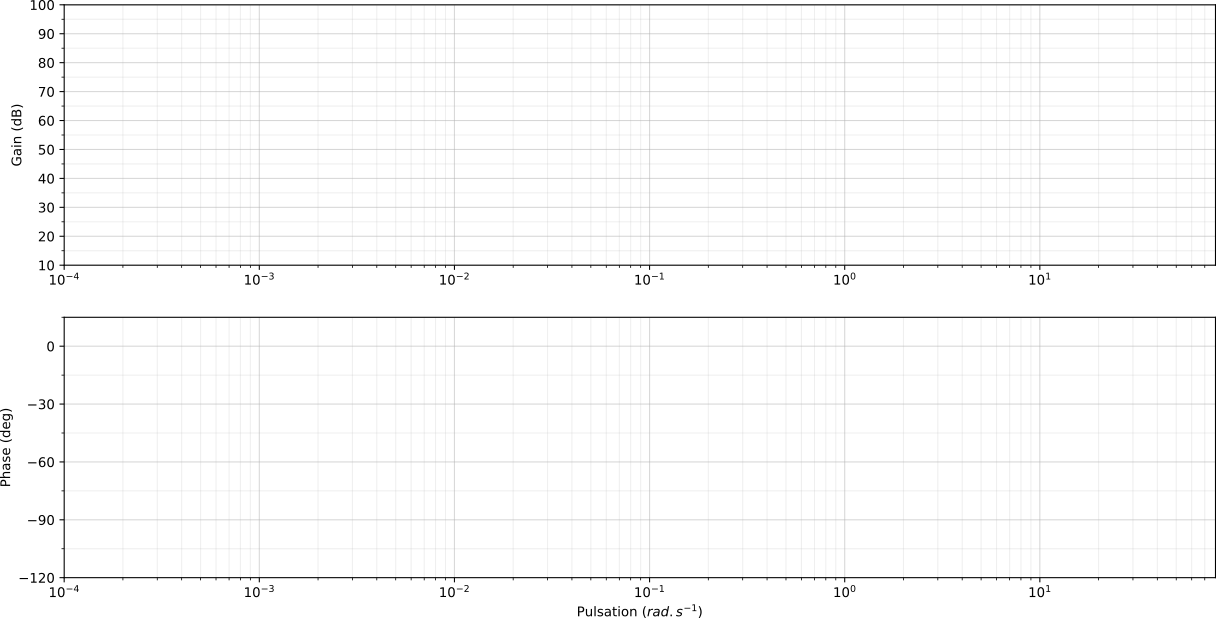
\includegraphics[width=\linewidth]{img/Bode_3}
\end{center}}{\begin{center}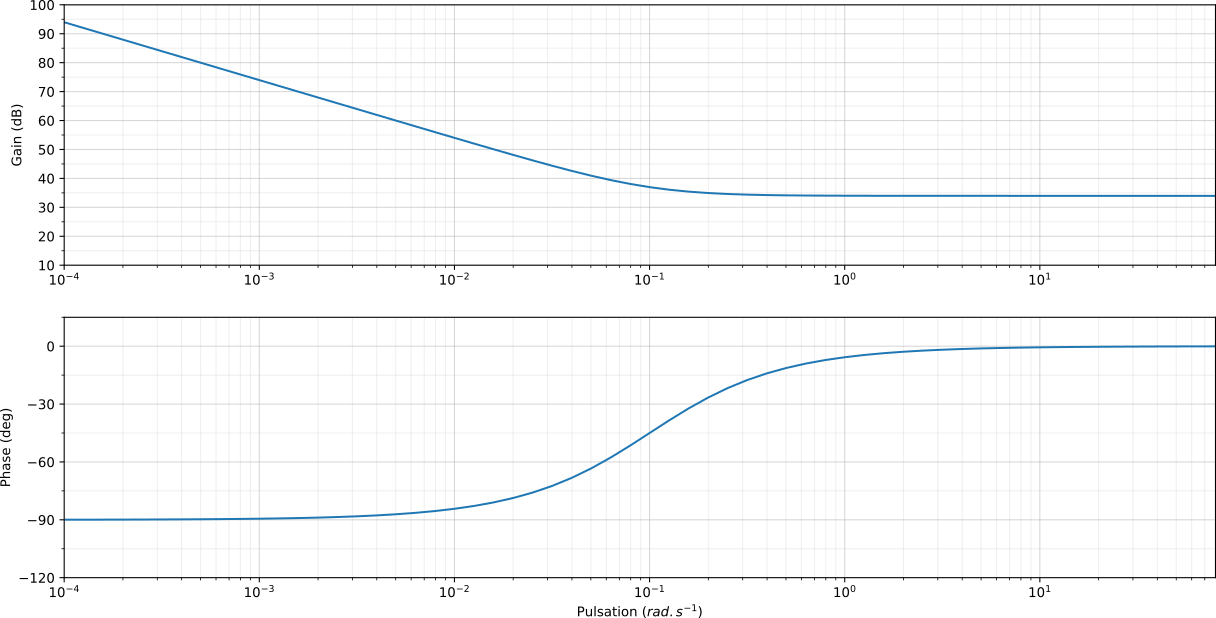
\includegraphics[width=\linewidth]{img/Bode_3_cor}
\end{center}}

\ifdef{\public}{\newpage}{}

\reponse{2}{}{Il s'agit d'une saturation.}

\reponse{5}{}{
$tan(\Phi)=\dfrac{MF}{MO_0}$ et $tan(q\cdot\Phi)=\dfrac{RM}{MO_0}$

Donc, $\dfrac{MF}{tan(\Phi)}=\dfrac{RM}{tan(q\cdot\Phi)}$
}

\reponse{4}{}{$RM+MF=L$, donc $RM=L\cdot\frac{tan(q\cdot\Phi)}{tan(\Phi)+tan(q\cdot\Phi)}$ et $MF=L\cdot\frac{tan(\Phi)}{tan(\Phi)+tan(q\cdot\Phi)}$
}

\reponse{4}{}{$tan(\Phi)=\dfrac{MF}{\rho}$ et $MF=L\cdot\frac{tan(\Phi)}{tan(\Phi)+tan(q\cdot\Phi)}$, donc 
$\rho=L\cdot\frac{1}{tan(\Phi)+tan(q\cdot\Phi)}$
}

\ifdef{\public}{\newpage}{}

\reponse{4}{}{
$tan(\Phi^{th}_g)=\dfrac{\frac{L}{2}}{\rho-\frac{v_a}{2}}$

Donc, $\rho=\dfrac{v_a}{2}+\dfrac{\frac{L}{2}}{tan(\Phi^{th}_g)}$

$tan(\Phi^{th}_d)=\dfrac{\frac{L}{2}}{\rho+\frac{v_a}{2}}$

Donc, $\rho=-\dfrac{v_a}{2}+\dfrac{\frac{L}{2}}{tan(\Phi^{th}_d)}$

Donc, $tan(\Phi^{th}_g)=\dfrac{L\cdot tan(\Phi^{th}_d)}{L-2\cdot v_a\cdot tan(\Phi^{th}_d)}$ et $tan(\Phi^{th}_d)=\dfrac{L\cdot tan(\Phi^{th}_g)}{L+2\cdot v_a\cdot tan(\Phi^{th}_g)}$}

\reponse{4}{}{$\overrightarrow{OI}+\overrightarrow{IB_g}+\overrightarrow{B_gC_g}+\overrightarrow{C_gD_g}+\overrightarrow{D_gO}=\overrightarrow{0}$

Donc, 
$-r\cdot \overrightarrow{y_1}-b\cdot\overrightarrow{x_1}-c\cdot\overrightarrow{x_{2g}}+d\cdot\overrightarrow{y_{3g}}+\dfrac{v_a}{2}\cdot\overrightarrow{x}-e\cdot\overrightarrow{y}=\overrightarrow{0}$

$\overrightarrow{OI}+\overrightarrow{IB_d}+\overrightarrow{B_dC_d}+\overrightarrow{C_dD_d}+\overrightarrow{D_dO}=\overrightarrow{0}$

Donc,
$-r\cdot\overrightarrow{y_1}+b\cdot\overrightarrow{x_1}+c\cdot\overrightarrow{x_{2d}}+d\cdot\overrightarrow{y_{3d}}-\dfrac{v_a}{2}\cdot\overrightarrow{x}-e\cdot\overrightarrow{y}=\overrightarrow{0}$
}


\reponse{0}{

~\ \\

$\left\{\begin{array}{l}
\overrightarrow{x_1}=\\
\overrightarrow{y_1}=\\
\overrightarrow{z_1}=
\end{array}\right.$

~\

$\left\{\begin{array}{l}
\overrightarrow{x_{2g}}=\\
\overrightarrow{y_{2g}}=\\
\overrightarrow{z_{2g}}=
\end{array}\right.$

~\

$\left\{\begin{array}{l}
\overrightarrow{x_{2d}}=\\
\overrightarrow{y_{2d}}=\\
\overrightarrow{z_{2d}}=
\end{array}\right.$

~\

$\left\{\begin{array}{l}
\overrightarrow{x_{3g}}=\\
\overrightarrow{y_{3g}}=\\
\overrightarrow{z_{3g}}=
\end{array}\right.$

~\

$\left\{\begin{array}{l}
\overrightarrow{x_{3d}}=\\
\overrightarrow{y_{3d}}=\\
\overrightarrow{z_{3d}}=
\end{array}\right.$}{

~\

$\left\{\begin{array}{l}
\overrightarrow{x_1}=cos(\theta)\cdot\overrightarrow{x}+sin(\theta)\cdot\overrightarrow{y}\\
\overrightarrow{y_1}=-sin(\theta)\cdot\overrightarrow{x}+cos(\theta)\cdot\overrightarrow{y}\\
\overrightarrow{z_1}=\overrightarrow{z}
\end{array}\right.$

~\

$\left\{\begin{array}{l}
\overrightarrow{x_{2g}}=cos(\beta_g)\cdot\overrightarrow{x}+sin(\beta_g)\cdot\overrightarrow{y}\\
\overrightarrow{y_{2g}}=-sin(\beta_g)\cdot\overrightarrow{x}+cos(\beta_g)\cdot\overrightarrow{y}\\
\overrightarrow{z_{2g}}=\overrightarrow{z}
\end{array}\right.$

~\

$\left\{\begin{array}{l}
\overrightarrow{x_{2d}}=cos(\beta_d)\cdot\overrightarrow{x}+sin(\beta_d)\cdot\overrightarrow{y}\\
\overrightarrow{y_{2d}}=-sin(\beta_d)\cdot\overrightarrow{x}+cos(\beta_d)\cdot\overrightarrow{y}\\
\overrightarrow{z_{2d}}=\overrightarrow{z}
\end{array}\right.$

~\

$\left\{\begin{array}{l}
\overrightarrow{x_{3g}}=cos(\gamma_g)\cdot\overrightarrow{x}+sin(\gamma_g)\cdot\overrightarrow{y}\\
\overrightarrow{y_{3g}}=-sin(\gamma_g)\cdot\overrightarrow{x}+cos(\theta)\cdot\overrightarrow{y}\\
\overrightarrow{z_{3g}}=\overrightarrow{z}
\end{array}\right.$

~\

$\left\{\begin{array}{l}
\overrightarrow{x_{3d}}=cos(\gamma_d)\cdot\overrightarrow{x}+sin(\gamma_d)\cdot\overrightarrow{y}\\
\overrightarrow{y_{3d}}=-sin(\gamma_d)\cdot\overrightarrow{x}+cos(\gamma_d)\cdot\overrightarrow{y}\\
\overrightarrow{z_{3d}}=\overrightarrow{z}
\end{array}\right.$
}

\reponse{9}{}{

$-r\cdot \overrightarrow{y_1}-b\cdot\overrightarrow{x_1}-c\cdot\overrightarrow{x_{2g}}+d\cdot\overrightarrow{y_{3g}}+\dfrac{v_a}{2}\cdot\overrightarrow{x}-e\cdot\overrightarrow{y}=\overrightarrow{0}$

$-r\cdot (-sin(\theta)\cdot\overrightarrow{x}+cos(\theta)\cdot\overrightarrow{y})-b\cdot(cos(\theta)\cdot\overrightarrow{x}+sin(\theta)\cdot\overrightarrow{y})-c\cdot(cos(\beta_g)\cdot\overrightarrow{x}+sin(\beta_g)\cdot\overrightarrow{y})+d\cdot(-sin(\gamma_g)\cdot\overrightarrow{x}+cos(\gamma_g)\cdot\overrightarrow{y})+\dfrac{v_a}{2}\cdot\overrightarrow{x}-e\cdot\overrightarrow{y}=\overrightarrow{0}$

$-r\cdot\overrightarrow{y_1}+b\cdot\overrightarrow{x_1}+c\cdot\overrightarrow{x_{2d}}+d\cdot\overrightarrow{y_{3d}}-\dfrac{v_a}{2}\cdot\overrightarrow{x}-e\cdot\overrightarrow{y}=\overrightarrow{0}$

$-r\cdot(-sin(\theta)\cdot\overrightarrow{x}+cos(\theta)\cdot\overrightarrow{y})+b\cdot(cos(\theta)\cdot\overrightarrow{x}+sin(\theta)\cdot\overrightarrow{y})+c\cdot(cos(\beta_d)\cdot\overrightarrow{x}+sin(\beta_d)\cdot\overrightarrow{y})+d\cdot(-sin(\gamma_d)\cdot\overrightarrow{x}+cos(\gamma_d)\cdot\overrightarrow{y})-\dfrac{v_a}{2}\cdot\overrightarrow{x}-e\cdot\overrightarrow{y}=\overrightarrow{0}$
}

\reponse{9}{}{

$r\cdot sin(\theta)-b\cdot cos(\theta)-c\cdot cos(\beta_g)-d\cdot sin(\gamma_g)+\dfrac{v_a}{2}=0$

$-r\cdot cos(\theta)-b\cdot sin(\theta)-c\cdot sin(\beta_g)+d\cdot cos(\gamma_g)-e=0$

$\beta_g=arccos\left(\dfrac{r\cdot sin(\theta)-b\cdot cos(\theta)-d\cdot sin(\gamma_g)+\dfrac{v_a}{2}}{c}\right)$

$-r\cdot cos(\theta)-b\cdot sin(\theta)-c\cdot sin\left(arccos\left(\dfrac{r\cdot sin(\theta)-b\cdot cos(\theta)-d\cdot sin(\gamma_g)+\dfrac{v_a}{2}}{c}\right)\right)+d\cdot cos(\theta)-e=0$

$r\cdot sin(\theta)+b\cdot cos(\theta)+c\cdot cos(\beta_d)-d\cdot sin(\gamma_d)-\dfrac{v_a}{2}=0$

$-r\cdot cos(\theta)+b\cdot sin(\theta)+c\cdot sin(\beta_d)+d\cdot cos(\gamma_d)-e=0$

$\beta_d=arccos\left(\dfrac{-r\cdot sin(\theta)-b\cdot cos(\theta)+d\cdot sin(\gamma_d)+\dfrac{v_a}{2}}{c}\right)$

$-r\cdot cos(\theta)+b\cdot sin(\theta)+c\cdot sin\left(arccos\left(\dfrac{-r\cdot sin(\theta)-b\cdot cos(\theta)+d\cdot sin(\gamma_d)+\dfrac{v_a}{2}}{c}\right)\right)+d\cdot cos(\gamma_d)-e=0$

}
\end{document}
